% Chapter 1

\chapter{Introduction} % Main chapter title

\label{Chapter1} % For referencing the chapter elsewhere, use \ref{Chapter1} 

%----------------------------------------------------------------------------------------

% Define some commands to keep the formatting separated from the content 
\newcommand{\keyword}[1]{\textbf{#1}}
\newcommand{\tabhead}[1]{\textbf{#1}}
\newcommand{\code}[1]{\texttt{#1}}
\newcommand{\file}[1]{\texttt{\bfseries#1}}
\newcommand{\option}[1]{\texttt{\itshape#1}}

\newcommand{\ts}{\textsuperscript}
\newcommand{\caII}{Ca II H \& K\xspace}
\newcommand{\Rprime}{$R^{'}_{HK}$\xspace}
\newcommand{\Smw}{$S_{MW}$\xspace}

\newcommand{\esp}{\textit{ESPaDOnS}\xspace}
\newcommand{\narval}{\textit{NARVAL}\xspace}
\newcommand{\Halpha}{H-$\alpha$\xspace}

\newcommand{\Ro}{$R_{0}$\xspace}
\newcommand{\tauc}{$\tau_{c}$\xspace}

%----------------------------------------------------------------------------------------

\epigraph{\itshape Measure what is measurable, and make measurable what is not so.}{---Galileo Galilei}

\section{Motivation}

There are many wondrous sights to see in the night sky, but one sight in particular may be considered to be more extraordinary than all others - the aurora borealis or aurora australis (depending on which hemisphere you live in). More commonly known as the northern or southern lights respectively, this phenomena displays vivid colours in the night sky (as shown in Figure \ref{fig:aurora_from_space}) that move and evolve in time, eventually disappearing. The northern lights are caused by particles that originate from the Sun and travel towards earth, interacting with molecules in the upper atmosphere. These molecules are excited by the solar particles and emit light when they return to their relaxed state causing the aurora. The solar particles are carried away from the Sun in the solar wind \citep{Parker_1958} which requires an open magnetic field line typically found in sunspots or coronal holes which are both forms of magnetic activity (or lack thereof).

The link between aurora and magnetic activity dates back to the 1800's when a powerful solar storm hit the Earth, this is now more commonly known as the Carrington event. Many sunspots were recorded in the month leading up to the event, but on the 1$^{st}$ of September Richard Carrington and Richard Hodgson both independently recorded observations of a flare that occurred on the Sun \citep{Carrington_1858,Hodgson_1859}. This flare was associated with a coronal mass ejection that travelled towards Earth, causing auroras to be seen around the world, even in countries that are typically too close to the equator to see such events. While there have been no subsequent events as powerful as the Carrington event, the coronal mass ejection in March of 1989 caused a power outage in Quebec city and serves as a powerful reminder of the potential disruption magnetic activity can cause on Earth. 

\begin{figure}
    \centering
    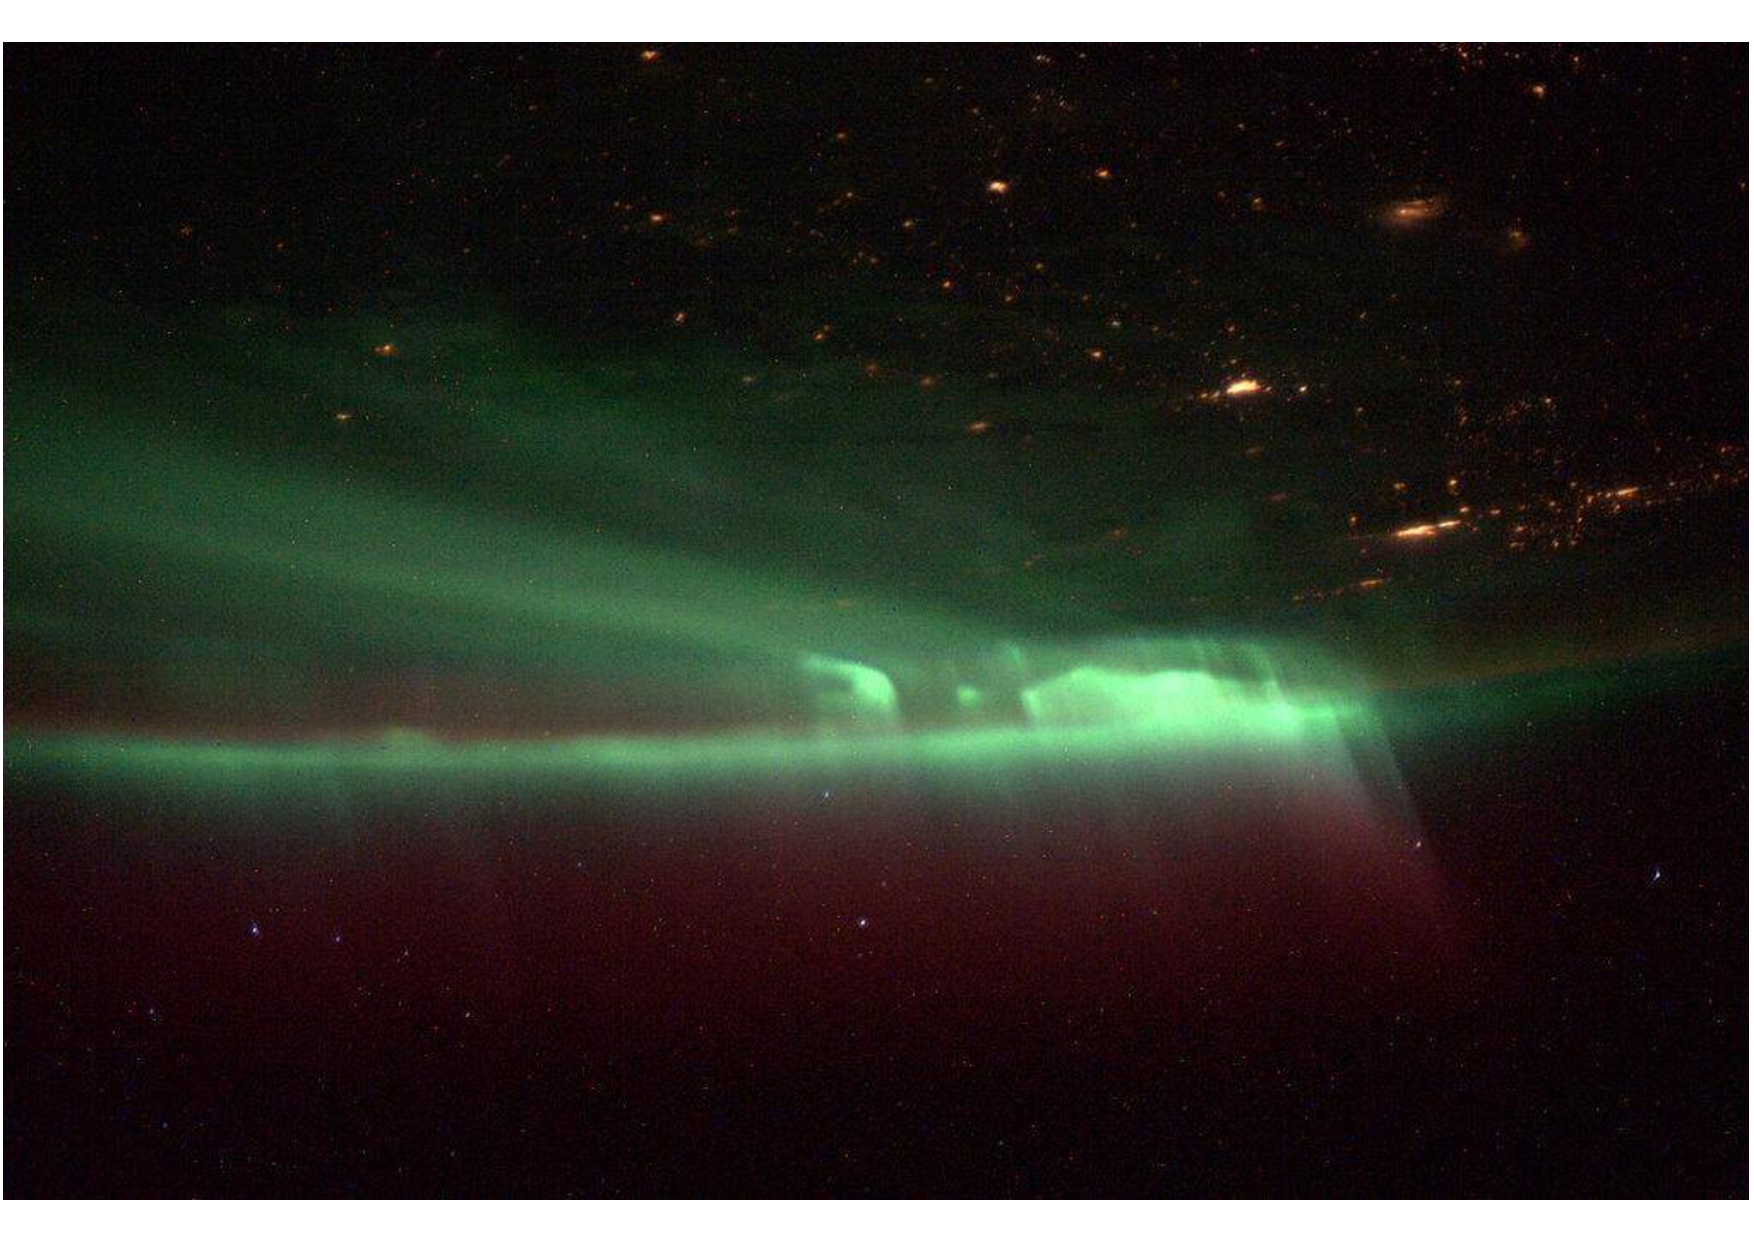
\includegraphics[scale=0.4]{Figures/1-Introduction/northern_lights_iss_20131009.pdf}
    \caption[Image of the northern lights as seen from space]{The northern lights as seen from space aboard the International Space Station. Image credt: NASA}
    \label{fig:aurora_from_space}
\end{figure}

'Magnetic activity' is a term that is used to describe a plethora of magnetically driven phenomena that occur on cool stars (spectral type F5 to mid-M) such as our own Sun. The study of solar magnetic activity dates back to the 17\ts{th} century when several scientists (Johannes Fabricius, Galileo Galilei and Christoph Scheiner) independently observed black spots on the Sun's surface. They found that these black spots (now known as sun spots) would move across the face of the Sun, disappearing off one side of the Sun and reappearing on the opposite side. This led the astronomers to believe that the Sun was moving and had a rotation period. These observations have led to over 400 years of studying the sun in detail and have given us a vast amount of information about how the Sun works. With the advancement of technology, we can now study the stars in our own Milky Way galaxy and try to establish how the Sun fits into the stellar population as a whole.

One may wonder how magnetic activity evolves in time, for example, what was the magnetic activity of the Sun like when life was just starting to evolve or what will it be like in the future? We could also ask what the magnetic activity is like on stars of varying stellar masses; this is particularly important when considering the potential habitability of an exoplanet (that is a planet that orbits another star other than our own Sun). It is these questions that are considered in the work presented in this thesis by considering the age-activity relationship. While the concept of the age-activity relationship is not new science, there are limitations to previous studies and regimes where the relationship can be improved upon. The difficulty with studying the evolution of stellar properties with time is that the ages of the stars must be known and this is not a trivial value to calculate. While many studies use clusters as calibration data set, these tend to be younger than a gigayear and there are very few older than this age. There are a handful clusters older than a gigayear but these tend to be more distant which makes calculation of magnetic activity indicators more difficult. The work presented in this thesis will attempt to extend the current knowledge of these age relationships by using ages determined from asteroseismology which has become a valuable technique in determining the ages of field stars.

To begin, I will give an overview of several topics that are crucial in the understanding of the age-activity relationship. These topics include:stellar dynamo and magnetic braking (Section \ref{Section:intro_dynamo_and_braking_section}), the stellar atmosphere and the magnetic activity associated with each region (Section \ref{Section:intro_stellar_structure}) and the ages of stars and methods to determine them (Section \ref{Section:intro_ages}).

\section{Stellar dynamo and magnetic braking}
\label{Section:intro_dynamo_and_braking_section}

\subsection{Stellar Dynamo Theory}
The first observation of solar magnetic fields was by \citet{Hale_1908}, where the Zeeman effect was observed in the spectrum of a sunspot. The Zeeman effect describes the interaction between atoms and the magnetic field \citep{Zeeman_1897}; the electronic energy levels of an atom will split when exposed to a magnetic field causing multiple absorption/emission spectral lines. Whereas only one spectral line would be present without a magnetic field. This raises the question, how does the Sun produce its magnetic field? The answer lies within the interior structure of the Sun; the Sun has a radiative core surrounded by a convective envelope. It is the interaction of these two layers at the tachocline that allows the magnetic field to be produced (known as the dynamo effect) and magnetic activity to be observed. This dynamo action is also seen in stars with spectral type ranging from F5 to $\approx$ M3 - M4, as these stars have a similar structure the Sun but with differing volumes of convective zone. Below a stellar mass of $\approx 0.35 M_{\odot}$, stars are expected to be fully convective and no longer have a radiative zone \citep{Chabrier_1997}. It is therefore theorised that a different type of dynamo operates in these stars that does not require a radiative zone (e.g. \citealt{Durney_etal_1993}) and is still an active research topic in the community. Conversely, stars with spectral types earlier than F5 do not have a substantial outer convective envelope that is required for the solar-like dynamo process \citep{Pinsonneault_etal_2001}.

The theory of the solar dynamo is described by magnetohydrodynamics (MHD), this is the study of the magnetic properties and behaviour of fluids that are electrically conducting such as plasma in stars. While the full details of the solar dynamo are not fully understood as it is an active topic of research, the most accepted theory is the $\alpha\Omega$ dynamo \citep{Choudhuri_2007}. If we consider an ordinary electromagnetic dynamo, a conducting coil rotates in a magnetic field and cuts through magnetic flux lines thus producing an electromotive force (e.m.f.) by Faraday's Law of induction. In stars, there are rotating regions of plasma that can also induce an e.m.f. and in favourable conditions the e.m.f. can reinforce the magnetic field. Therefore, the dynamo process can build up a magnetic field starting from an initial seed field. This initial seed field comes from the gas cloud that the star formed from since observations of gas clouds do have a magnetic field associated with them. It is known that the Sun does not rotate as a solid body but rather the equator spins $\approx 20 \%$ faster than the poles. This is an important factor in dynamo theory as it can also be shown that the magnetic field is frozen in the plasma and moves with it, this is Alfve\'n's theorem of flux-freezing \citep{Alfven_1942}. It is because of differential rotation and flux freezing that the poloidal magnetic field is then stretched out in the toroidal direction, this is shown in the middle panel of Figure \ref{fig:dynamo} and is known as the $\Omega$ effect. This $\Omega$ effect takes place in the region where differential rotation is at its greatest: helioseismology has found that this region is known as the tachocline and is located at the bottom of the convection zone. Therefore, it is expected that the strongest toroidal field will be at the tachocline.

\begin{figure}
    \centering
    \captionsetup{width=.9\linewidth}
    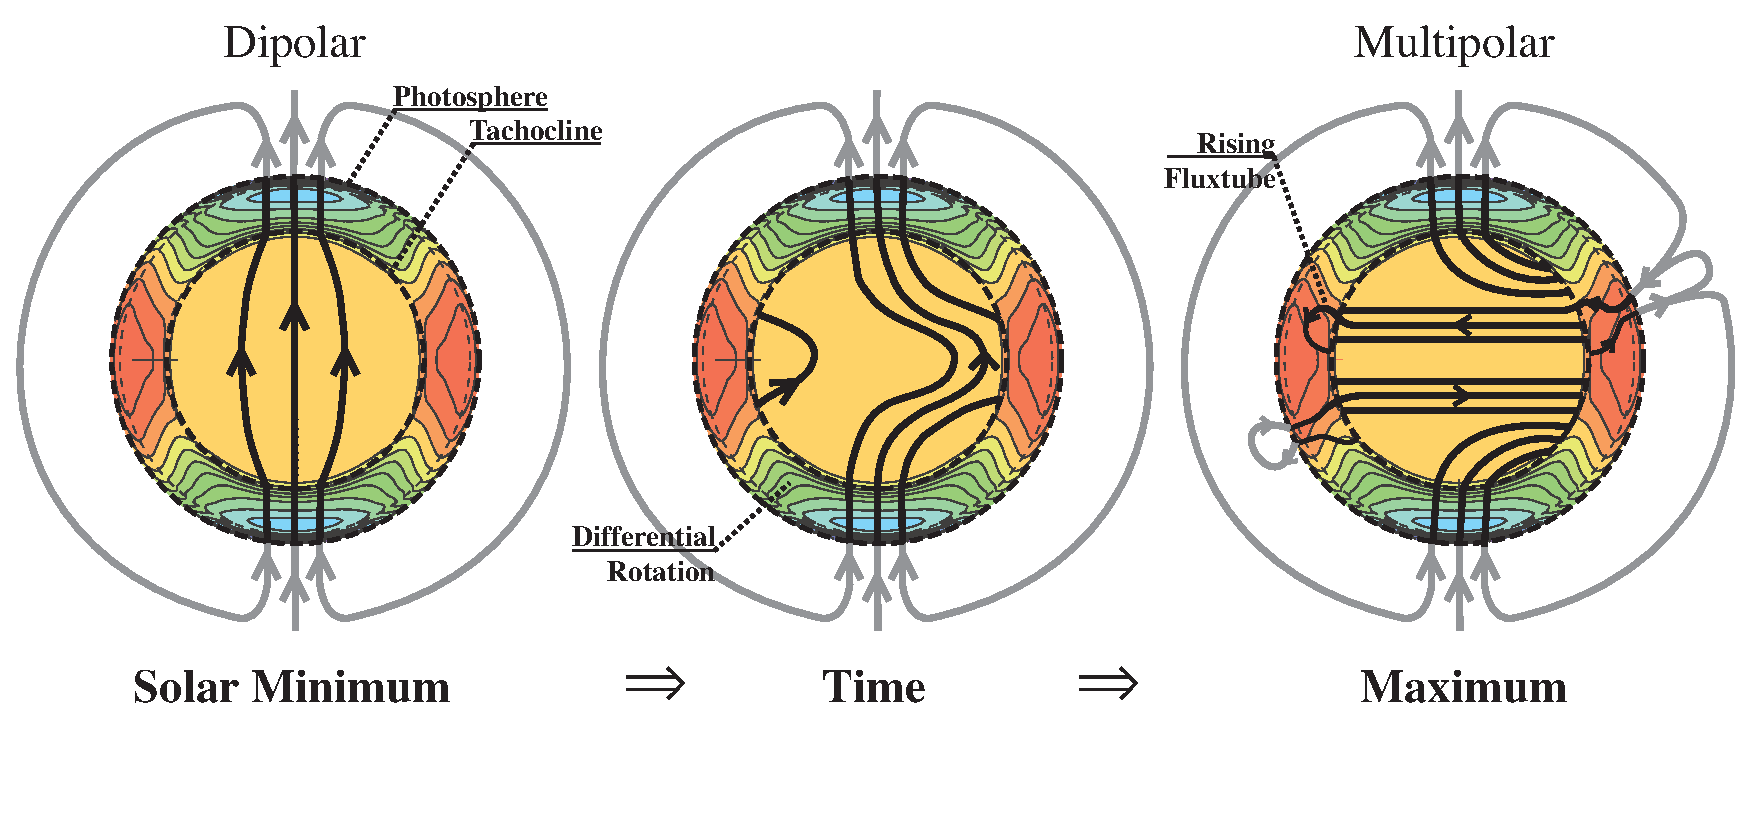
\includegraphics[width=.9\linewidth]{Figures/1-Introduction/dynamo_schem.eps}
    \caption[Schematic of the solar dynamo]{A schematic of the solar dynamo, it shows the interior and magnetic field lines of the Sun over time from solar minimum to solar maximum. The colours show the rate of rotation within the Sun where the red indicates a faster rate of rotation and blue indicates a slower rate of rotation. Over time the differential rotation in the convection zone causes the poloidal field to be stretched in the toroidal direction. As the magnetic fields become sheared and twisted they become "flux-ropes" and magnetic buoyancy causes them to rise to the solar surface. At solar maximum these flux-ropes appear at the solar surface, making the solar magnetic field to become multipolar. Image courtesy of \citet{higgins_2012}}
    \label{fig:dynamo}
\end{figure}

Another important aspect of the solar dynamo is the interaction of the magnetic field with the convection in the plasma (known as magnetoconvection). Numerical simulations by \citet{Weiss_1981} studied the nonlinear evolution of convection in the presence of a magnetic field; they found that two different regions formed. In the first region, magnetic field is excluded and vigorous convection takes place. In the second region, the magnetic field gets concentrated and the tension of the magnetic field lines suppresses convection. In the latter regions, flux tubes form which are concentrated bundles of magnetic field lines. In regions of strong differential rotation (such as the tachocline), these flux tubes will align with the toroidal field and if they have magnetic buoyancy, they can rise to the surface of the star. Flux tubes that pierce the solar surface can the form bipolar spots, these are spots close together with opposite polarities. From these sunspots, some of the toroidal magnetic field is converted back into poloidal field but the exact mechanism is still an open question.

The most likely mechanism is known as the Babcock-Leighton mechanism \citep{Babcock_1961,Leighton_1969}. It is known that bipolar spots have a tilt associated with them that increases with increasing latitude (known as Joy's Law), therefore one spot is closer to the equator than the other. Each spot diffuses its polarity at different latitudes which then forms a poloidal field at the solar surface. These field lines then migrate towards the pole through the meridional circulation which is the constant flow of plasma near the Sun's surface from the equator to the pole. The field lines can then flow to the tachocline from the poles by the counterpart to the meridional circulation which must exists as we do not not observe an excess of material at the pole. Thus completes the solar dynamo cycle and the process can repeat.

\subsection{Angular momentum evolution of stars}

All stars are formed with an initial amount of angular momentum that comes from the formation process, but the angular momentum is not constant over the lifetime of the star. In this section I will give a brief overview of how the angular momentum changes throughout a solar-type star's lifetime. Figure \ref{fig:gallet_&_bouvier_2013_fig} shows the angular velocity as a function of age for solar type stars in star-forming regions and young open clusters. The large distribution of angular velocities in these stars is due to the initial angular momentum that each star was born with. However, once solar-type stars reach $\approx 1$ Gyr, they converge to a similar angular velocity.

\begin{figure}[h]
    \centering
    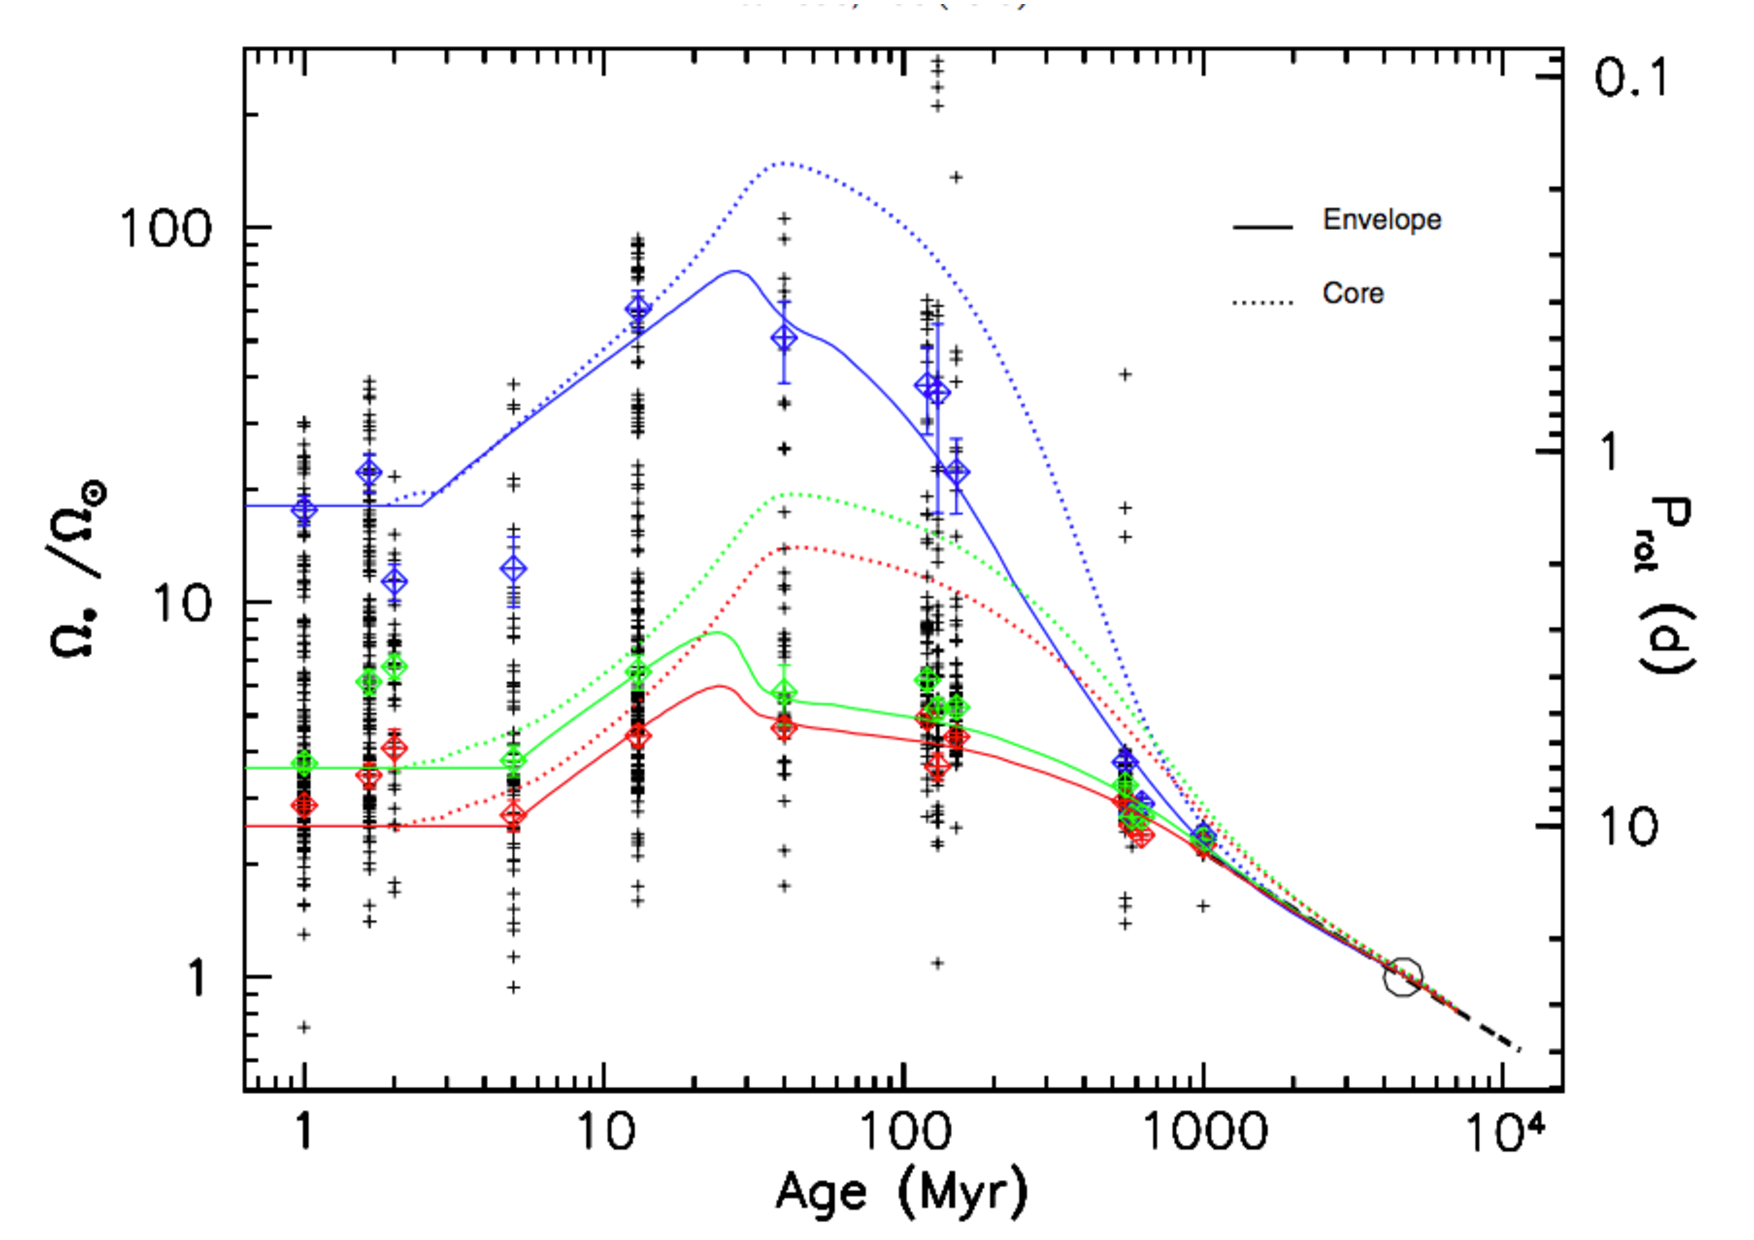
\includegraphics[scale=0.4]{Figures/1-Introduction/gallet&_bouvier_figure_2013.pdf}
    \caption[Angular velocity distribution as a function of age]{Figure from \citet{Gallet_Bouvier_2013} that shows the angular velocity distribution of solar-type stars in star-forming regions and young open clusters as a function of age. Also plotted are the angular velocity of the radiative core (dashed lines) and convective envelope (solid lines) as a function of time for fast (blue), median (green) and slow (red) rotator models. The open circle represents the angular velocity of the Sun. The black dashed line represents the Skumanich law.}
    \label{fig:gallet_&_bouvier_2013_fig}
\end{figure}

During the pre-main-sequence (PMS), despite the fact that these stars are still contracting from their formation, they are prevented from spinning up due to interactions with their accretion disk \citep{Edwards_etal_1993,Rebull_etal_2004}. This period lasts for a few million years until the accretion disk disappears. The star then continues to spin up due to contraction from its formation until it reaches the zero age main sequence (ZAMS). Once the star is on the main sequence (MS) then angular momentum is lost from its magnetised stellar wind in a process called magnetic braking.

An important aspect of the models shown in Figure \ref{fig:gallet_&_bouvier_2013_fig} is the distribution of angular momentum within the interior of the stars. If a star has strong core-envelope coupling then the whole star reacts to angular momentum that is lost at the stellar surface resulting in a long-term steady decline of the surface velocity. Whereas in decoupled models, the radiative core retains most of the initial angular momentum while the convective envelope may lose angular momentum. Then at later times in the decoupled model, the angular momentum stored in the core of these stars can be redistributed to the convective envelope thus delaying the spin down phase. It is the key difference between the fast and median/slow rotator models. In fast rotator models, the core-envelope coupling has a relatively short timescale of 12 Myr. In contrast, the slow and median rotator models have a core-envelope coupling timescale of 28-30 Myr which allows the convective envelope to be efficiently braked before the ZAMS. The core-envelope coupling also explains the difference in shape of the rotational tracks, slow and median rotators have a much flatter rotational evolution on the the early MS as angular momentum is being slowly transferred back into the envelope from the core.

The work in this thesis focuses on the angular momentum lost while solar and late-type stars are on the the main sequence. \citet{Schatzman_1962} first proposed that stars could lose angular momentum through their magnetised stellar wind. Material that is lost from the stellar surface (e.g. through solar wind or flares) is forced to co-rotate with the stellar surface by the magnetic field up until a critical distance, known as the Alfve\'n radius. The Alfve\'n radius is defined as the point where the magnetic energy density is equal to the kinetic energy density, beyond this point the material is said to be lost from the star and carries away some angular momentum. The rate at which the star loses angular momentum depends on several factors: the strength of the magnetic field, the initial rotational velocity, the velocity and density of the wind and the length of time over which the process occurs on \citep{Weber_&_Davis_1967}. Since the generation of the magnetic field is linked to the rotation of the star through the stellar dynamo, as the star loses angular momentum we expect both the rotation period and magnetic activity of the star to decrease with time. This has led to many studies on the evolution of these parameters with age, which will be discussed in Chapter \ref{Chapter2}. Consequently, the change in the magnetic field of the star will also affect the efficiency of the magnetic braking.

\section{Stellar atmosphere and magnetic activity}
\label{Section:intro_stellar_structure}

All stars form from clouds of gas and dust that collapse under its own gravitational force, the centre of the cloud becomes hotter and more dense until the correct conditions are met for nuclear fusion to begin and a star is born. While all stars are essentially astronomical bodies that burn hydrogen into helium at its core (at some stage in their life), the mass of the star has a strong influence over the structure of the star and consequently its evolution. In this work, I concentrate my studies on stars with spectral type ranging from F5 to $\approx$ M3 ($1.33 M_{\odot} - 0.35 M_{\odot}$) because the structure of these stars allows for the manifestation of magnetic activity. These solar-and late-type stars have a radiative core surrounded by a convective envelope, it is the interaction of these two layers that allows the magnetic field to be produced (see Section \ref{Section:intro_dynamo_and_braking_section}) and magnetic activity to be observed. Therefore, any further discussion about stellar structure will be in relation to this range of the stellar population. Magnetic activity is observed from the atmosphere of a star where we define the atmosphere as the region where photons can escape directly into space. In this section, I will outline the different layers of the solar atmosphere and the types of magnetic activity seen in each region. I will mainly focus on solar observations as we can resolve the surface of the Sun and this allows us to study the phenomena in greater detail.

\subsection{Photosphere}

The lowest part of the solar atmosphere is known as the photosphere, it is only several hundred kilometres thick yet is the region that emits most of the solar radiation. This is the part of the Sun that we can see with our naked eye and is commonly referred to as the "surface" of the Sun. The surface of the Sun is defined at the optical depth of $\tau = 1$. Optical depth is a measure of the transparency of a medium and is defined by Equation \ref{Eq:optical_depth_eq} where $I$ is the amount of outgoing radiation, $I_{0}$ is the amount of incident radiation and $\tau$ is the optical depth. Therefore, at an optical depth of one, the radiation has fallen by a factor $e$.

\begin{equation}
    I = I_{0}e^{-\tau}
    \label{Eq:optical_depth_eq}
\end{equation}

The main diagnostic for magnetic activity in the photosphere is sunspots, these are dark regions that appear on the surface of the Sun. They have been observed for many centuries, naked eye observations date back to 165 BC \citep{Wittmann_1987} while telescope observations started in 1611 with the rediscovery of sunspots by Galilei, Scheiner and others. Sunspots are characterised by three regions - a dark core, the umbra and the penumbra, an example of a complex sunspot is shown in Figure \ref{fig:sunspot_example}. Sunspots occur in active regions of the Sun where the magnetic field is more intense, this inhibits convection and reduces the effective temperature of that region compared to the surrounding photosphere (typically 2000 K cooler) thus appearing darker. The size and lifespan of sunspots are tied to the strength of the magnetic field therefore longer lasting spots typically have stronger associated magnetic fields. The typical lifetime of a spot on the Sun is on the order of hours to weeks and most last a stellar rotation \citep{Bradshaw_Hartigan_2014}.

\begin{figure}
    \centering
    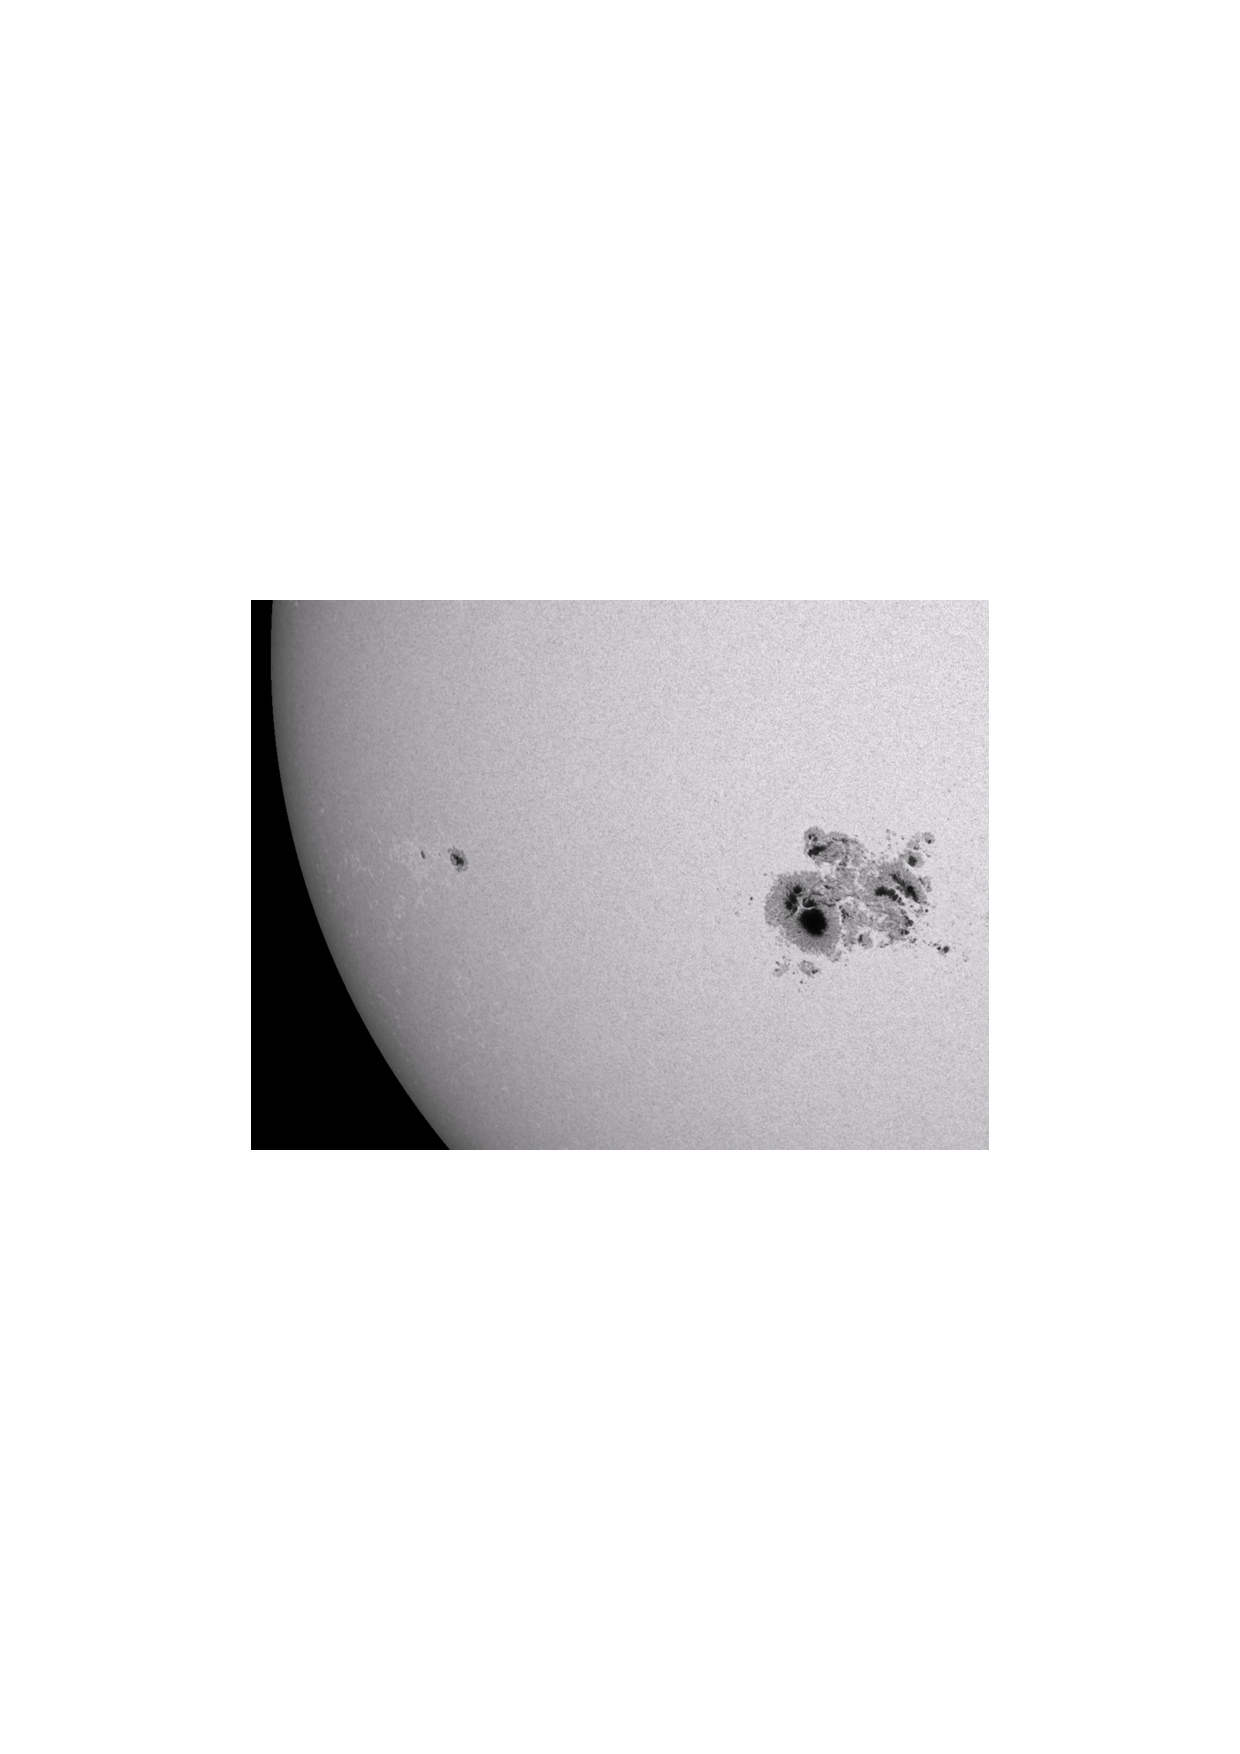
\includegraphics[scale=0.7]{Figures/1-Introduction/HMI_spot_Oct}
    \caption[Example of complex sunspot as seen by NASA's SDO]{Large, complex sunspot seen from NASA's Solar Dynamics Observatory from October 2014. Image Credit: NASA/SDO and the AIA, EVE, and HMI science teams.}
    \label{fig:sunspot_example}
\end{figure}

The observations of sunspots have lead to a better understanding of some of the internal processes at work within the solar interior. As early as the 1800's scientists were noticing patterns in the way sunspots evolved in time. \citet{Schwabe_1844} found that the occurrence of spot groups and spotless days repeated with a period of approximately 10 years, the modern day value of this period is 11 years and is known as the Schwabe solar cycle (or more commonly - the solar cycle). \citet{Carrington_1858} noticed that sunspots seemed to appear at different latitudes over time and this was later visualised by \citet{Maunder_1904} in the now infamous "butterfly diagram". An example of such a diagram is shown in Figure \ref{fig:butterfly_diagram}, we see that at the start of each solar cycle sunspots tend to form at mid-latitudes and migrate towards the equator over time.

\begin{figure}
    \centering
    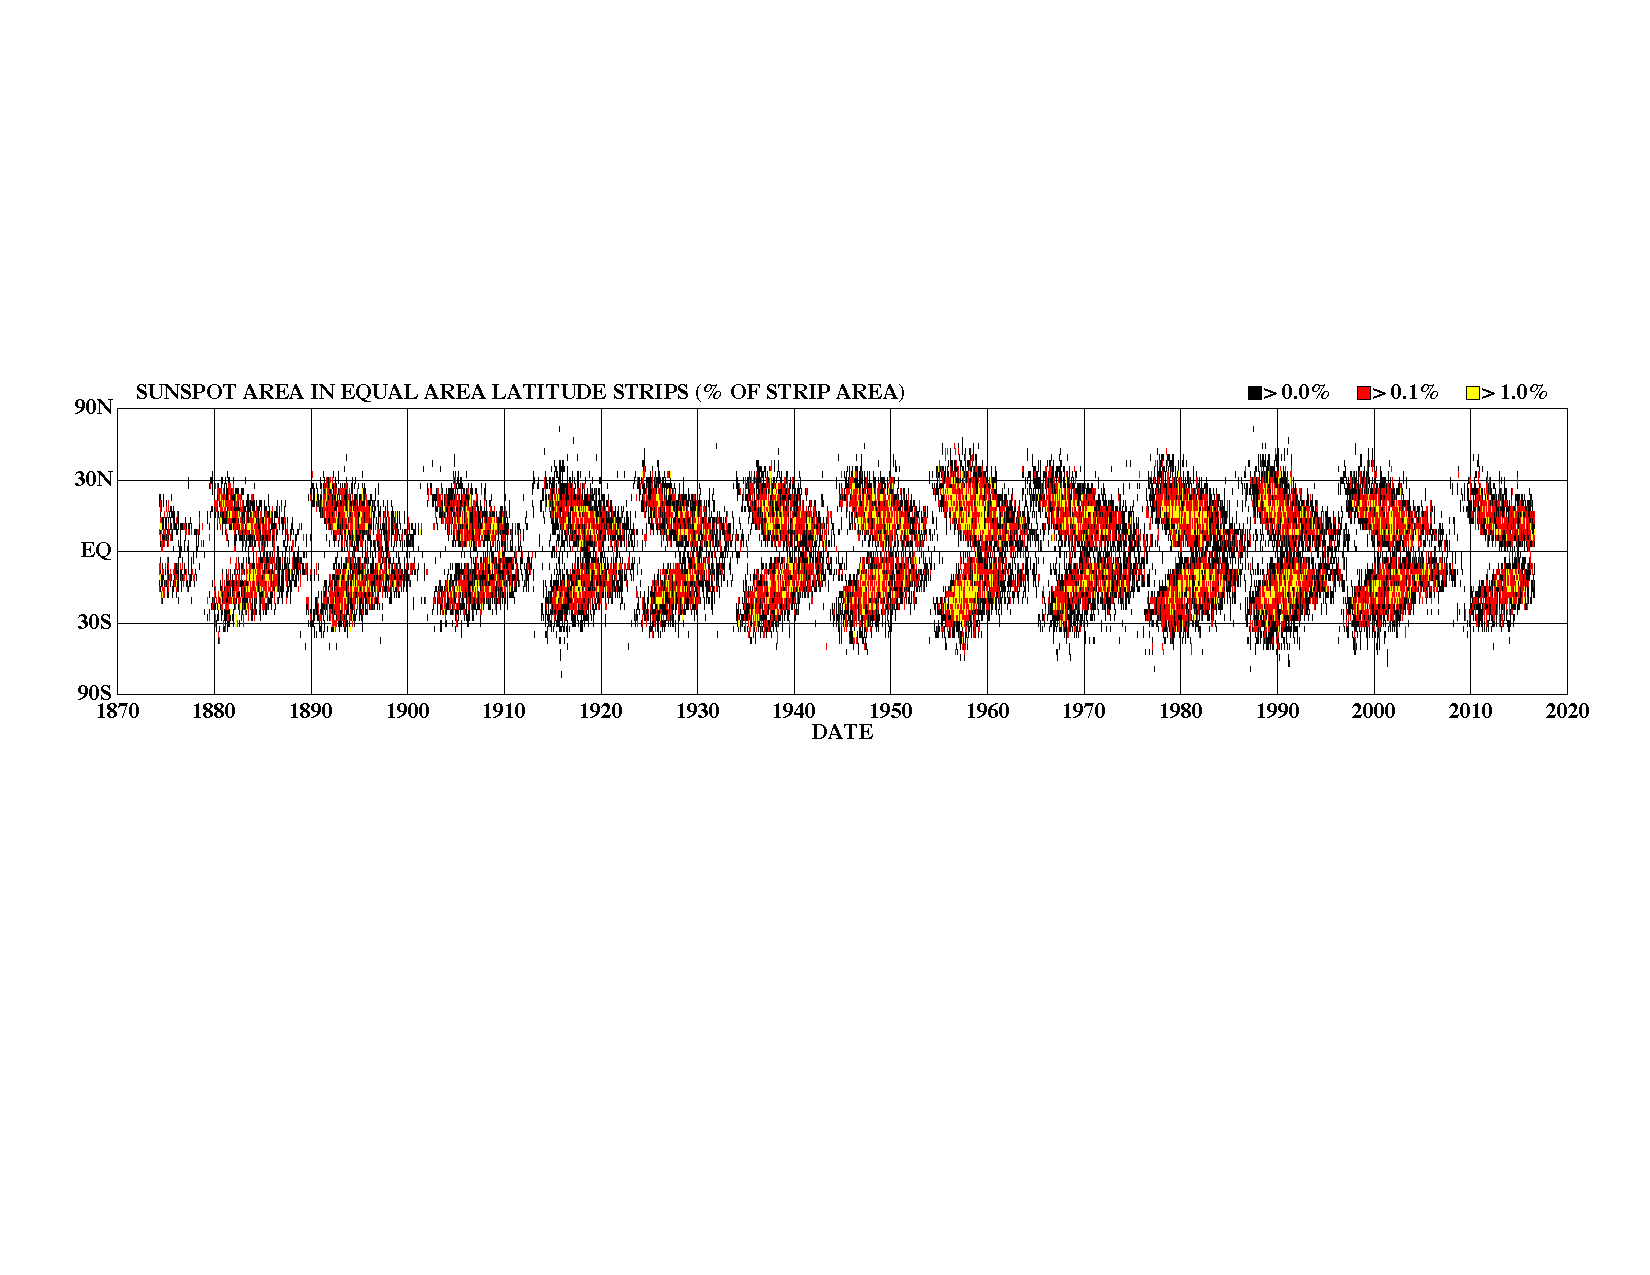
\includegraphics[scale=0.5]{Figures/1-Introduction/butterfly_diagram_crop.pdf}
    \caption[Butterfly diagram showing the latitudes of sunspots over a solar cycle]{An example of a butterfly diagram that shows the latitude of the sunspot as a function of time. At the start of each cycle, spots tend to form at mid-latitudes migrate towards the equator. Image credit: https://solarscience.msfc.nasa.gov/SunspotCycle.shtml}
    \label{fig:butterfly_diagram}
\end{figure}

One paper in particular noted several patterns that would become useful constraints for solar dynamo theories. \citet{Hale_etal_1919} devised a method of determining the angle between the magnetic field vector on the Sun and the line-of-sight which allowed the polarity of sunspots to be investigated. Firstly, they found that spots would frequently appear in pairs with the preceding member forming first, however there were exceptions to this rule. Secondly, the axis of a binary spot group formed a small angle with the equator, with the leading spot closest to the equator. This angle also tended to increase for higher latitudes, this is now known as Joy's Law. Thirdly, the two members of a binary spot group would be of opposite polarity. The polarity of the leading/following spot would be the same for bipolar spots in the same hemisphere, and would be the opposite for bipolar spots in the other hemisphere; this is known as Hale's Law. Lastly, after the solar cycle minimum, the polarity for the leading/following members in bipolar spots reverses in each hemisphere. This is known as the Hale magnetic cycle and comprises of two solar cycles.

\begin{figure}
    \centering
    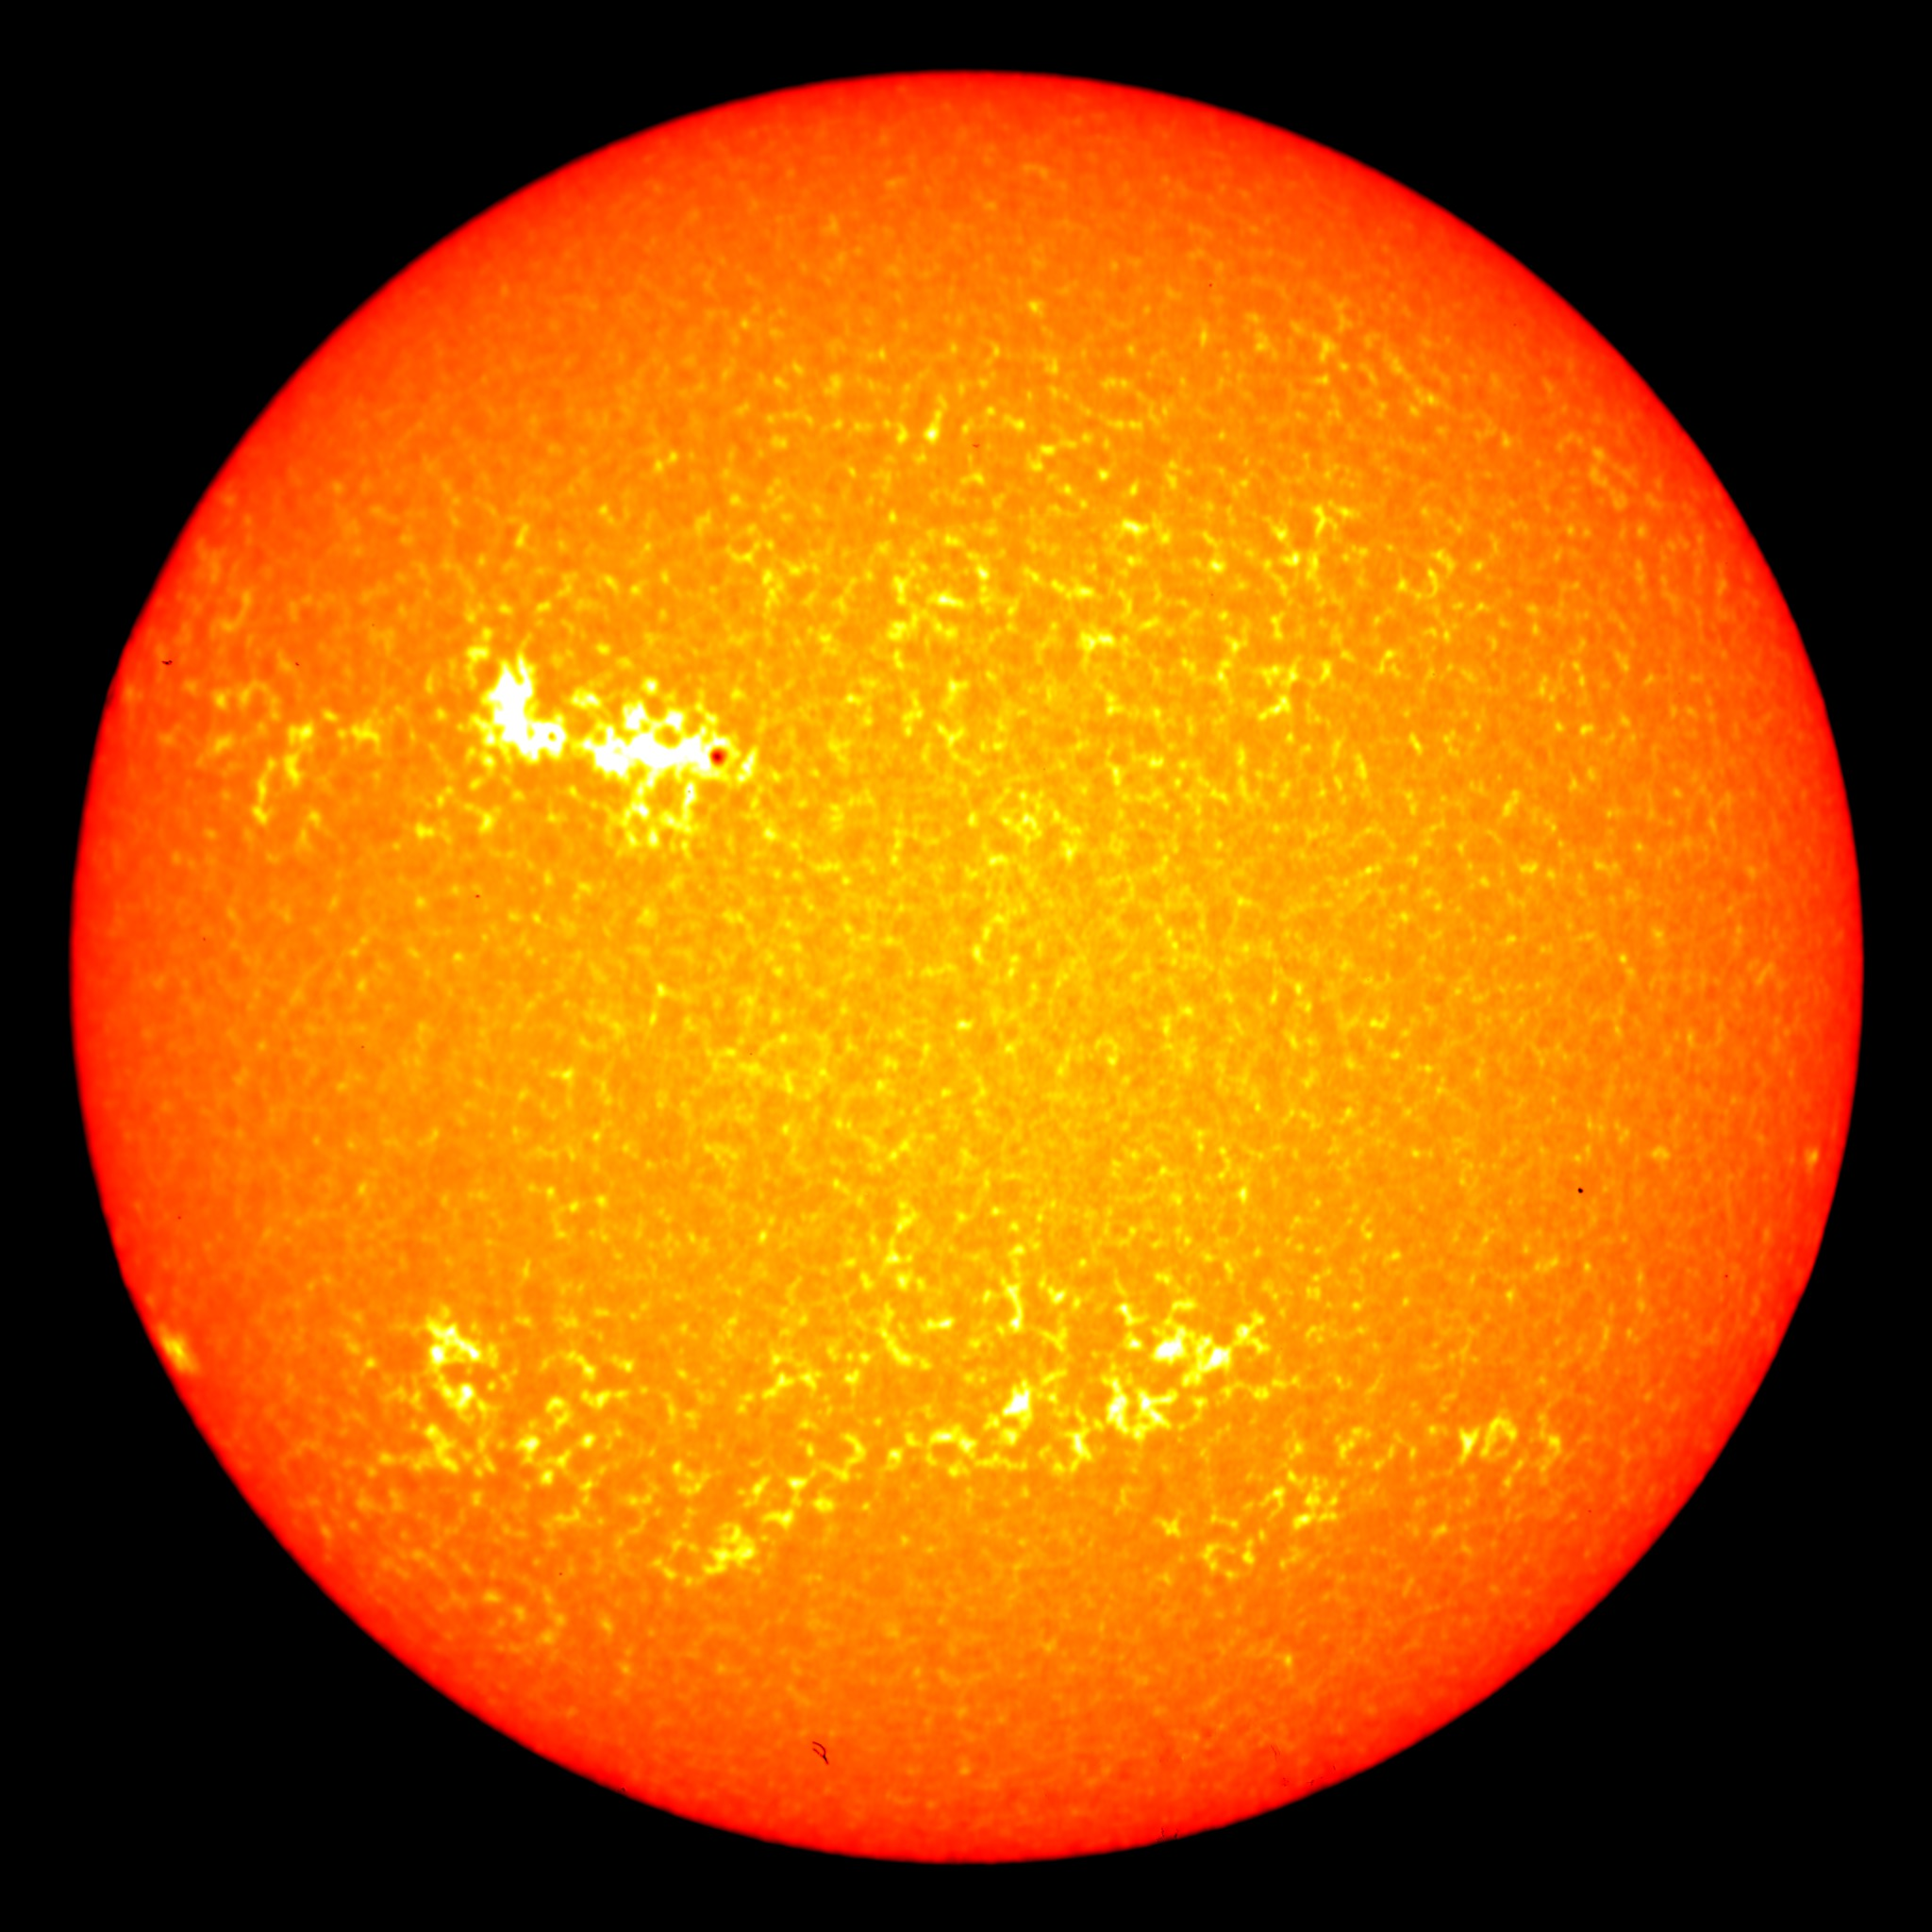
\includegraphics[scale=0.15]{Figures/1-Introduction/faculae_example.jpg}
    \caption[Example of faculae during a period of low activity on the Sun]{View of the Sun during a period of low activity in October 1998. Colour table has been altered to enhance the appearance of faculae which are seen as the bright white regions. Faculae appear near a small sunspot and in other regions with no sunspots. Image credit: NASA/Goddard Space Flight Center Scientific Visualization Studio. Source data courtesy of HAO \& NSO PSPT project team.}
    \label{fig:faculae_example}
\end{figure}

Another magnetic feature present in the photosphere are bright, small-scale regions known as faculae \citep{Hale_1922}. While faculae and plage are both spatially associated and the two terms are used synonymously they form in different stellar regions; faculae form in the photosphere while plage forms in the chromosphere. Faculae are regions of increased magnetic field, however it is not strong enough to inhibit convection as the case is for sunspots. Instead, the increased magnetic field alters the opacity at the surface allowing for a deeper view into the photosphere where it is hotter and therefore brighter. Faculae have a lower contrast with the surrounding photosphere, therefore they are best viewed near the limb of the Sun. Figure \ref{fig:faculae_example} shows an image of the Sun during a period of low activity in October 1998 (note that the colour table has been altered in order to enhance the appearance of faculae). The faculae are shown as bright white regions and we see that they appear near a small sunspot in the northern hemisphere but also appear in the southern hemisphere where no sunspots are present. Since there is a lower magnetic field threshold for faculae, they tend to be loner-lived and more abundant across the stellar disc than sunspots. This means that during solar maximum, there are large number of faculae resulting in an increase in the solar irradiance \citep{Walton_etal_2003}.

\subsection{Chromosphere}
The chromosphere is the region that lies above the photosphere and is approximately 2000km thick. Awareness of the Sun's atmosphere started through observations during solar eclipses; it was only during these events that the light form the photosphere was obscured and the light from the atmosphere could be revealed. The chromosphere is seen as a pink ring of emission at the solar limb and is only visible for a few seconds during an eclipse.

\begin{figure}
    \centering
    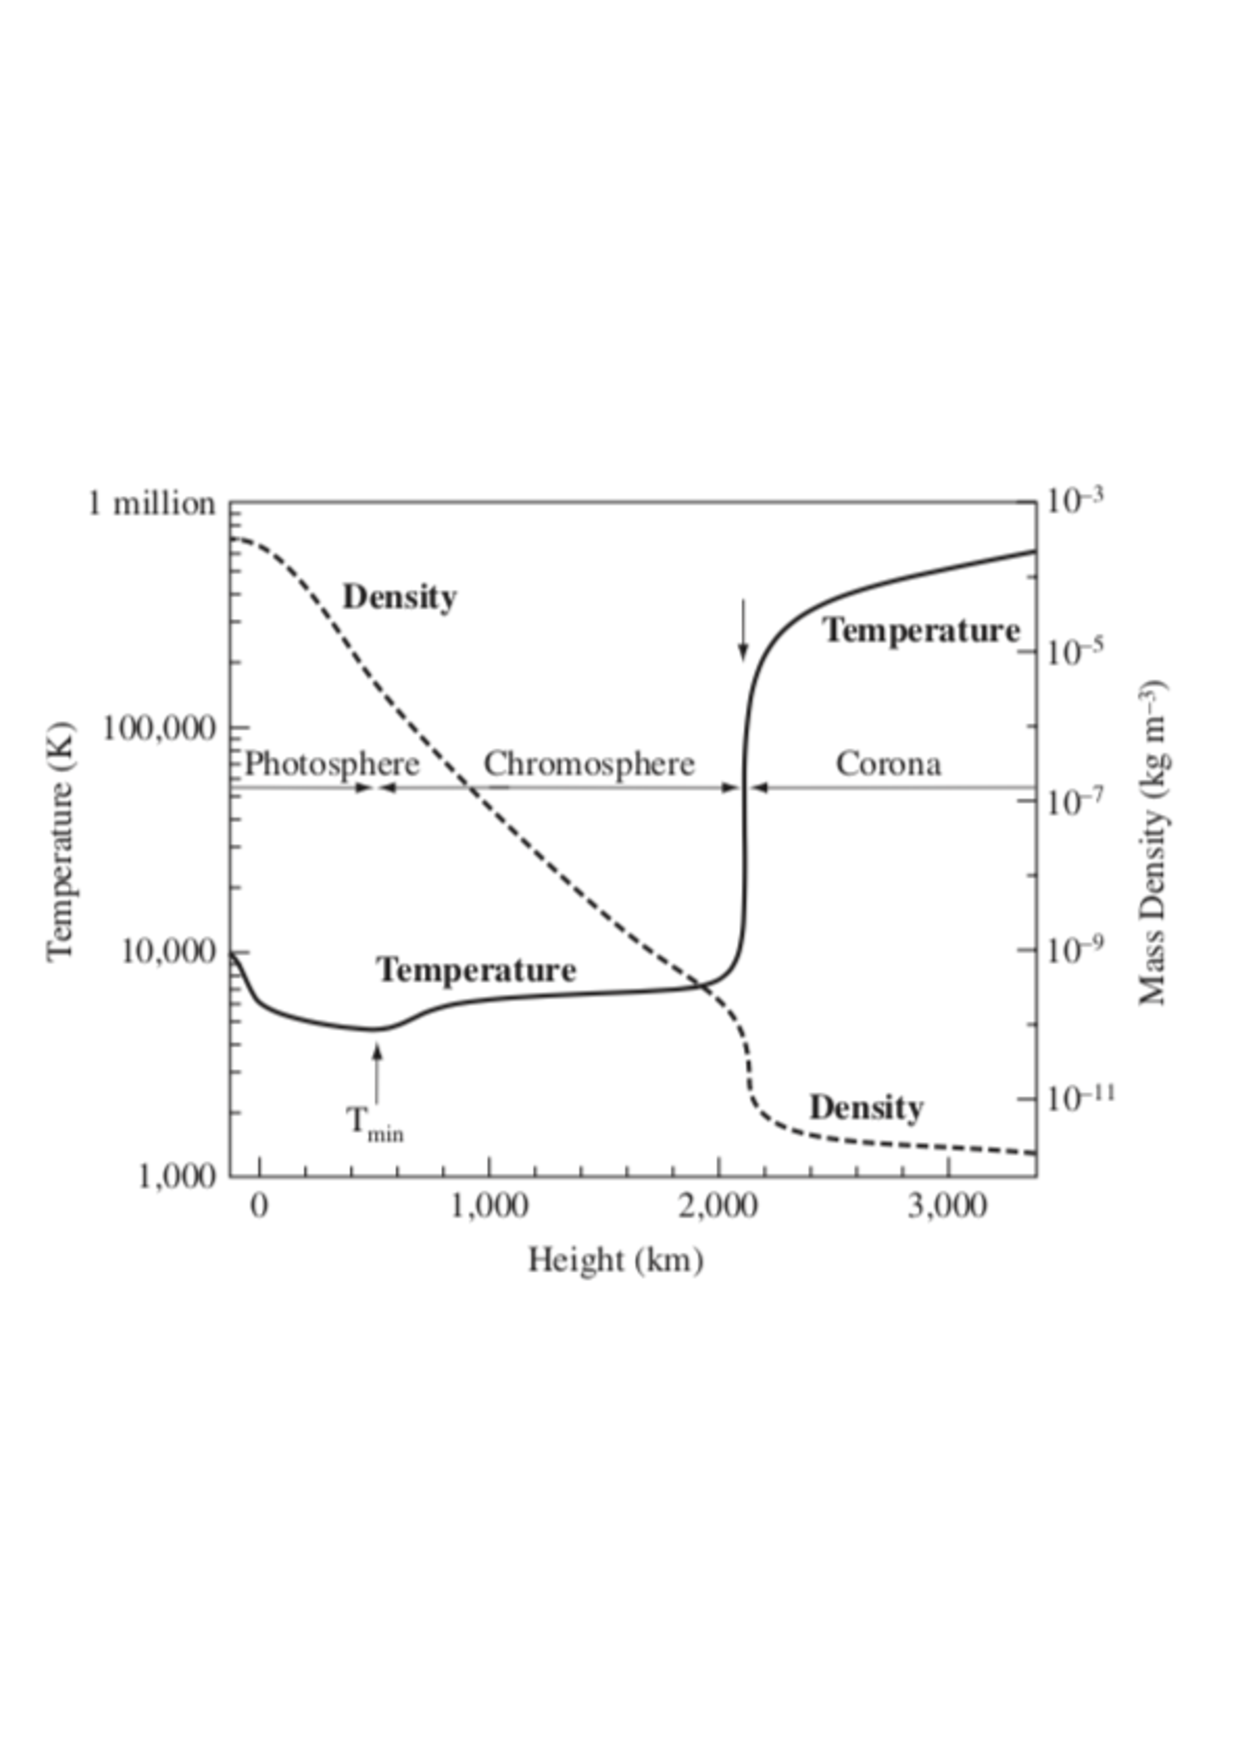
\includegraphics[scale=0.5]{Figures/1-Introduction/val_model_MHD_of_Sun_textbook.pdf}
    \caption[VAL model that shows the mean variation of temperature and density with height in the solar atmosphere]{Schematic of the mean variation of temperature and density with height in the solar atmosphere according to VAL model. Image credit: \citet{Priest_2014_MHD_sun}}
    \label{fig:val_model}
\end{figure}

Early work on the spectra of both the chromosphere and corona showed there were numerous emission features of ionised species that could only be present due to high temperatures. The temperature rises from $\approx$ 4400 K in the photosphere to 7000 K in the chromosphere and rises even further to 1,000,000 K in the corona. This is clearly seen in Figure \ref{fig:val_model} which shows the mean variation of temperature and density with height in the solar atmosphere according to a VAL model. The VAL model \citep{Vernazza_etal_1981} is a semi-empirical 1-D model that successfully fits a number of spectral lines from different regions but does have its limitations. The temperature rise seen in the chromosphere and corona cannot be explained by thermal processes alone, therefore there must be an additional heating mechanism at work. This is still an active topic of research but the most likely theories are MHD wave heating and magnetic reconnection \citep{Parnell_DeMoortel_2012}.

Magnetic features that appear in the chromosphere include spicules \citep{Roberts_1945} and their larger counterpart macrospicules \citep{Bohlin_etal_1975}. These are tight jets of plasma that stream upward through the chromosphere and are bright in H-$\alpha$. In addition to magnetic features that we can resolve on the Sun, since the chromosphere is heated by an additional magnetic process, we observe emission reversals in prominent Fraunhofer spectral lines such as \caII. The connection between calcium emission and the magnetic field has been known since \citet{Leighton_1959} found that plage corresponded to areas of calcium emission on the Sun. Studies of the calcium emission over the solar cycle also shows that it has a measurable difference (e.g. \citealt{White_Livingston_1981}) in comparisons to other parameters such as the solar irradiance. Another advantage of the emission from the \caII lines is that they are not sensitive to magnetic polarity therefore they are a good proxy for the total unsigned magnetic field \citep{Linsky_Avrett_1970}. Additional spectral lines also show chromospheric emission but the \caII spectral lines are by far the most commonly used.

 \subsection{Corona}
The outermost layer of the solar atmosphere is known as the corona, this is a region of very hot, low density gas. The first indirect evidence of the corona came from optical spectral lines of highly ionised elements \citep{Grotrian_1939} which indicated that these elements originated from a region with very high temperatures. It was not until the space age that we could fully investigate the corona as the majority of the emission occurs in wavelengths that are not observable from Earth such as extreme ultraviolet and X-rays; it wasn't until the invention of rockets that images of the Sun in these wavelengths could be taken (e.g. \citealt{van_Speybroeck_etal_1970}).

\begin{figure}
    \centering
    \includegraphics[scale=0.45]{Figures/1-Introduction/cor_hole_combo.pdf}
    \caption[UV image of Sun showing coronal features]{Image of the Sun in three different ultraviolet wavelengths from NASA's Solar Dynamics Observatory in January 2014. A large coronal hole that spans from the south polar region to mid latitudes is seen alongside several active regions that show coronal loops. Image credit: NASA/SDO and the AIA, EVE, and HMI science teams.}
    \label{fig:corona_structure}
\end{figure}

There are several key structures that appear in the corona; these include coronal holes, coronal loops and X-ray bright points. Coronal holes were first studied by \citet{Waldmeier_1956} but high-detailed images of them were not available until the 1970's \citep{Huber_etal_1974}. Coronal holes are the darkest and least active region of the Sun and are associated with open field lines and the acceleration of the solar-wind. Coronal holes are also some of the most long-lived features on the Sun as near solar minimum, large coronal holes cover the north and south polar caps and can last for 7-8 years; shorter-lived coronal holes can also appear at lower latitudes during solar minimum. Coronal loops are closed magnetic loops that are connected to photospheric bipolar regions. X-ray bright points are small yet intense features that are scattered around the whole disc. Examples of some of these features are seen in Figure \ref{fig:corona_structure} in ultraviolet wavelengths from NASA's SDO.

The corona also shows magnetic activity features such as flares and coronal mass ejections (CME's). Flares occur as a result of a relaxation in the magnetic field structure thus releasing magnetic energy that is radiated across the entire electromagnetic spectrum. CME's are large scale plasma bubbles that expand out from the Sun and cause major modifications in the large-scale structure of the corona. CME's are usually associated with other indicators of activity such as flares but do not necessarily occur together; generally weaker CME's occur without any flare-like manifestation however powerful flares do have associated CME's \citep{Andrews_2003}. The frequency of CME's depends on the phase of the solar cycle (as do other magnetic activity indicators); near solar maximum there can be up to 3.5 events per day while near solar minimum they can occur once every 5 days \citep{Carroll_Ostlie_2006}. In addition to the magnetic features, the overall X-ray flux that is emitted from the corona is a good indicator of magnetic activity since the corona is heated via magnetic fields. X-ray emission shows a good correlation with chromospheric indicators and the magnetic flux density (e.g. \citealt{Schrijver_etal_1992,Pevtsov_etal_2003}) thus making it a useful tool to study magnetic activity on other stars.

\subsection{Stellar magnetic activity}

Our proximity to the Sun has allowed use to observe it in exquisite detail, observing small-featured details such as spicules and granulation. In order to understand the Sun in a wider context, we must compare it to other stars within the galaxy yet we cannot resolve these stars in the same detail as we can for the Sun. However, we can still detect features of magnetic activity and this section will cover some of the ways that magnetic activity can be studied in other stars.

\subsubsection{Starspots}
\label{Chp1_starspots}
It stands to reason that since the Sun exhibits dark spots, other stars with a similar structure would also exhibit spots. Photometric observations of stars with starspots dates back to \citet{Kron_1947} when eclipsing binaries were studied and significant variation in the light curve was detected outside of the eclipse. It was theorised that this was due to light and dark patches on the surface of the star. Later \citet{Hall_1972} demonstrated that a model that included a region of starspot activity could reproduce the peculiarities in the data.

Since starspots move across the stellar surface at the same rate as the surface, the modulation in the light curve due to starspots can be used to determine the rotation period of the star. These rotation periods are much more reliable than measurements made from spectroscopic data as they are not dependent on the inclination of the star. To determine the rotation period, observations are needed over the timescale of the rotation period and ideally for several rotation periods; this means that observations tend to be bias towards faster rotators that have shorter rotation periods. In addition to this, observations are also bias towards younger stars as they are much more active than older stars therefore they have detectable modulations in photometric observations. However, progress is being made towards determining rotation periods for older and more slowly rotating stars (e.g. \citealt{Barnes_etal_2016,Douglas_etal_2016,Lanzafame_etal_2018}). Space telescopes such as Kepler/K2 have been instrumental in this progress as they continuously monitor stars for long periods of time and produce light curves spanning long periods of time that are ideal for determining rotation periods.

\begin{figure}
    \centering
    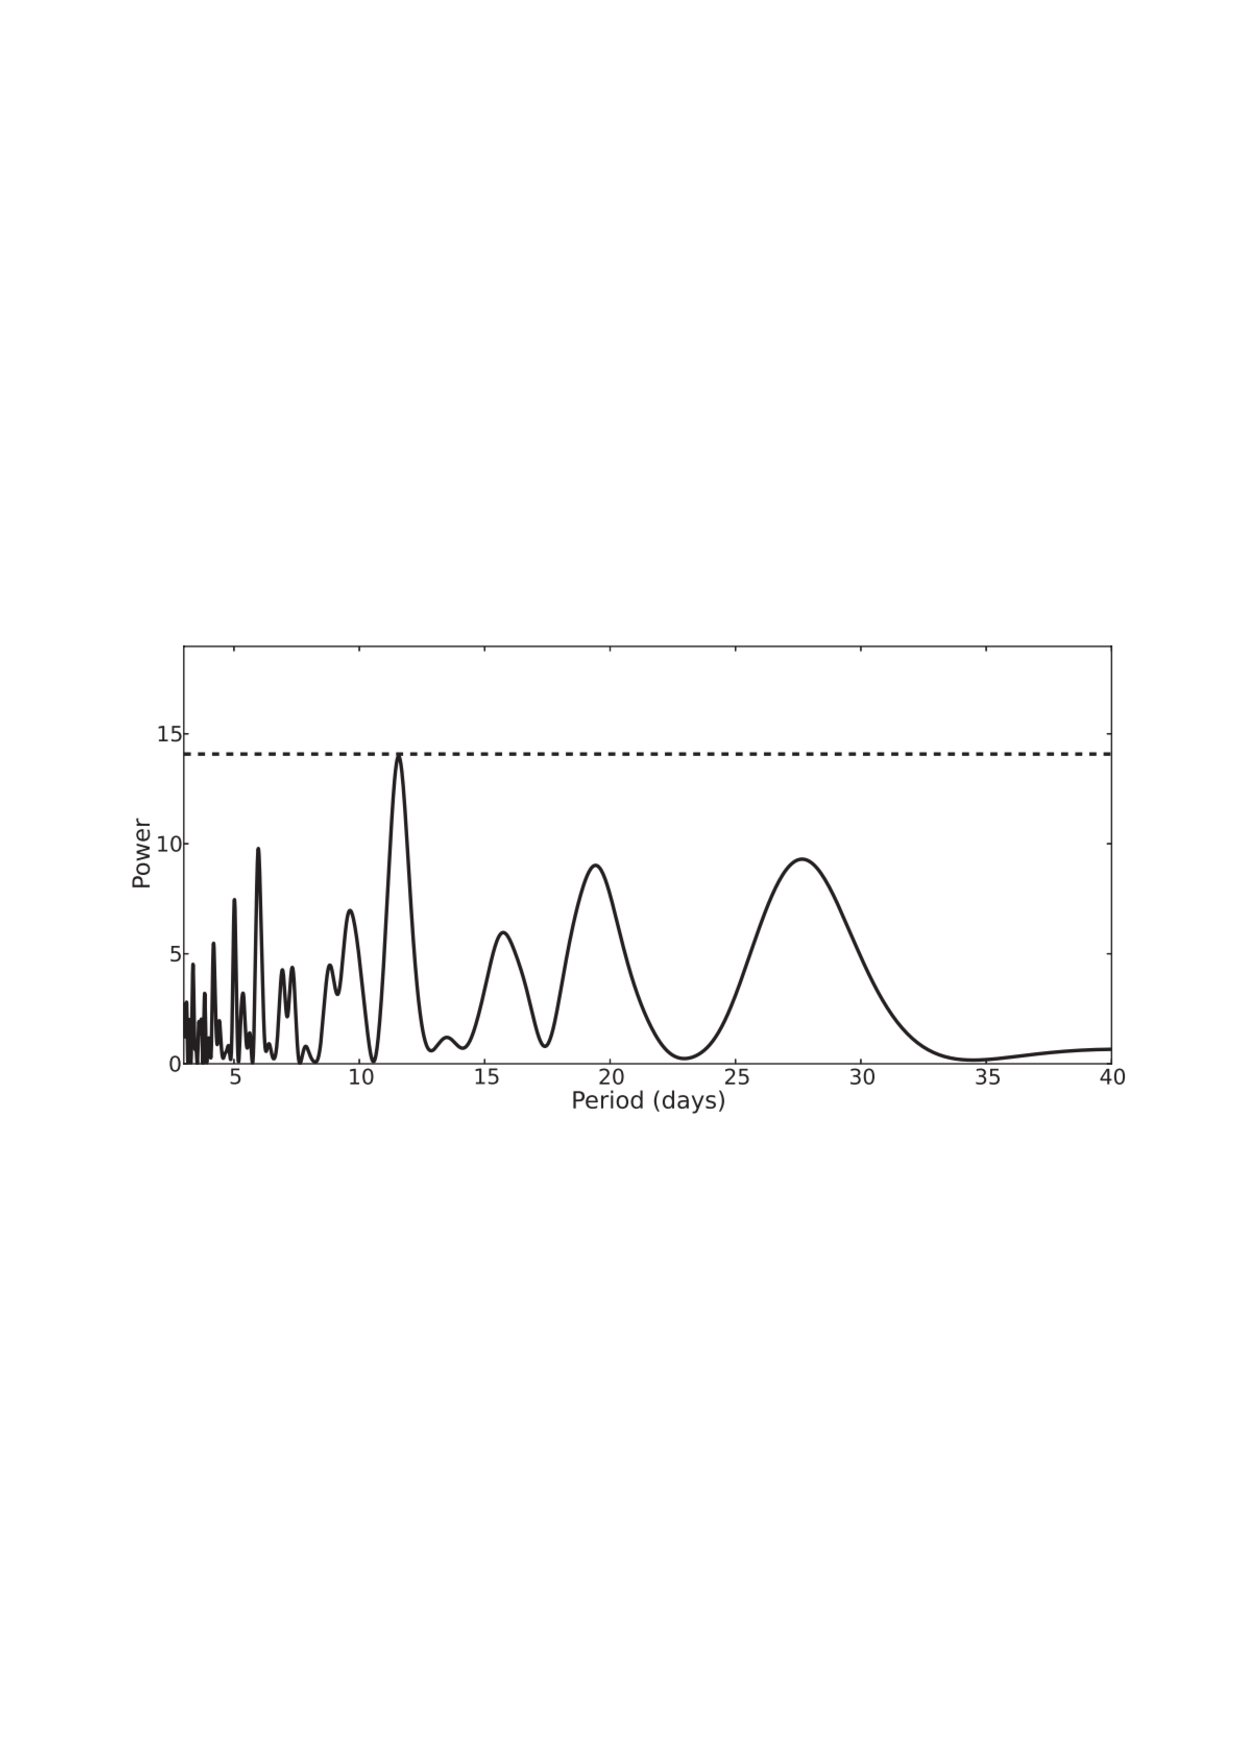
\includegraphics[scale=0.5]{Figures/1-Introduction/brothwell_2014_LSP.pdf}
    \caption[Lomb Scargle periodogram example]{Example of Lomb Scargle periodogram for the WASP 32 system. The dashed line represent the false alarm probability of 0.1 per cent. The peak period corresponds to a rotation period of 11.6 days. Image credit: \citet{Brothwell_etal_2014}}
    \label{fig:LS_periodogram_example}
\end{figure}

A common method of determining rotation periods from starspot modulation is to use a Lomb Scargle periodogram \citep{Lomb_1976,Scargle_1982}. This method takes a Fourier transform of the light curve to search for periodicities; since starspot modulations are sinusoidal in nature this will appear as a delta function in the Fourier transformation. Generally a distribution of delta peaks will appear in the power spectrum of the data similar to the example shown in Figure \ref{fig:LS_periodogram_example}. When considering the rotation period, it is appropriate to choose the period with the largest Lomb Scargle power \citep{Nielsen_Karoff_2012}.

\begin{figure}
    \centering
    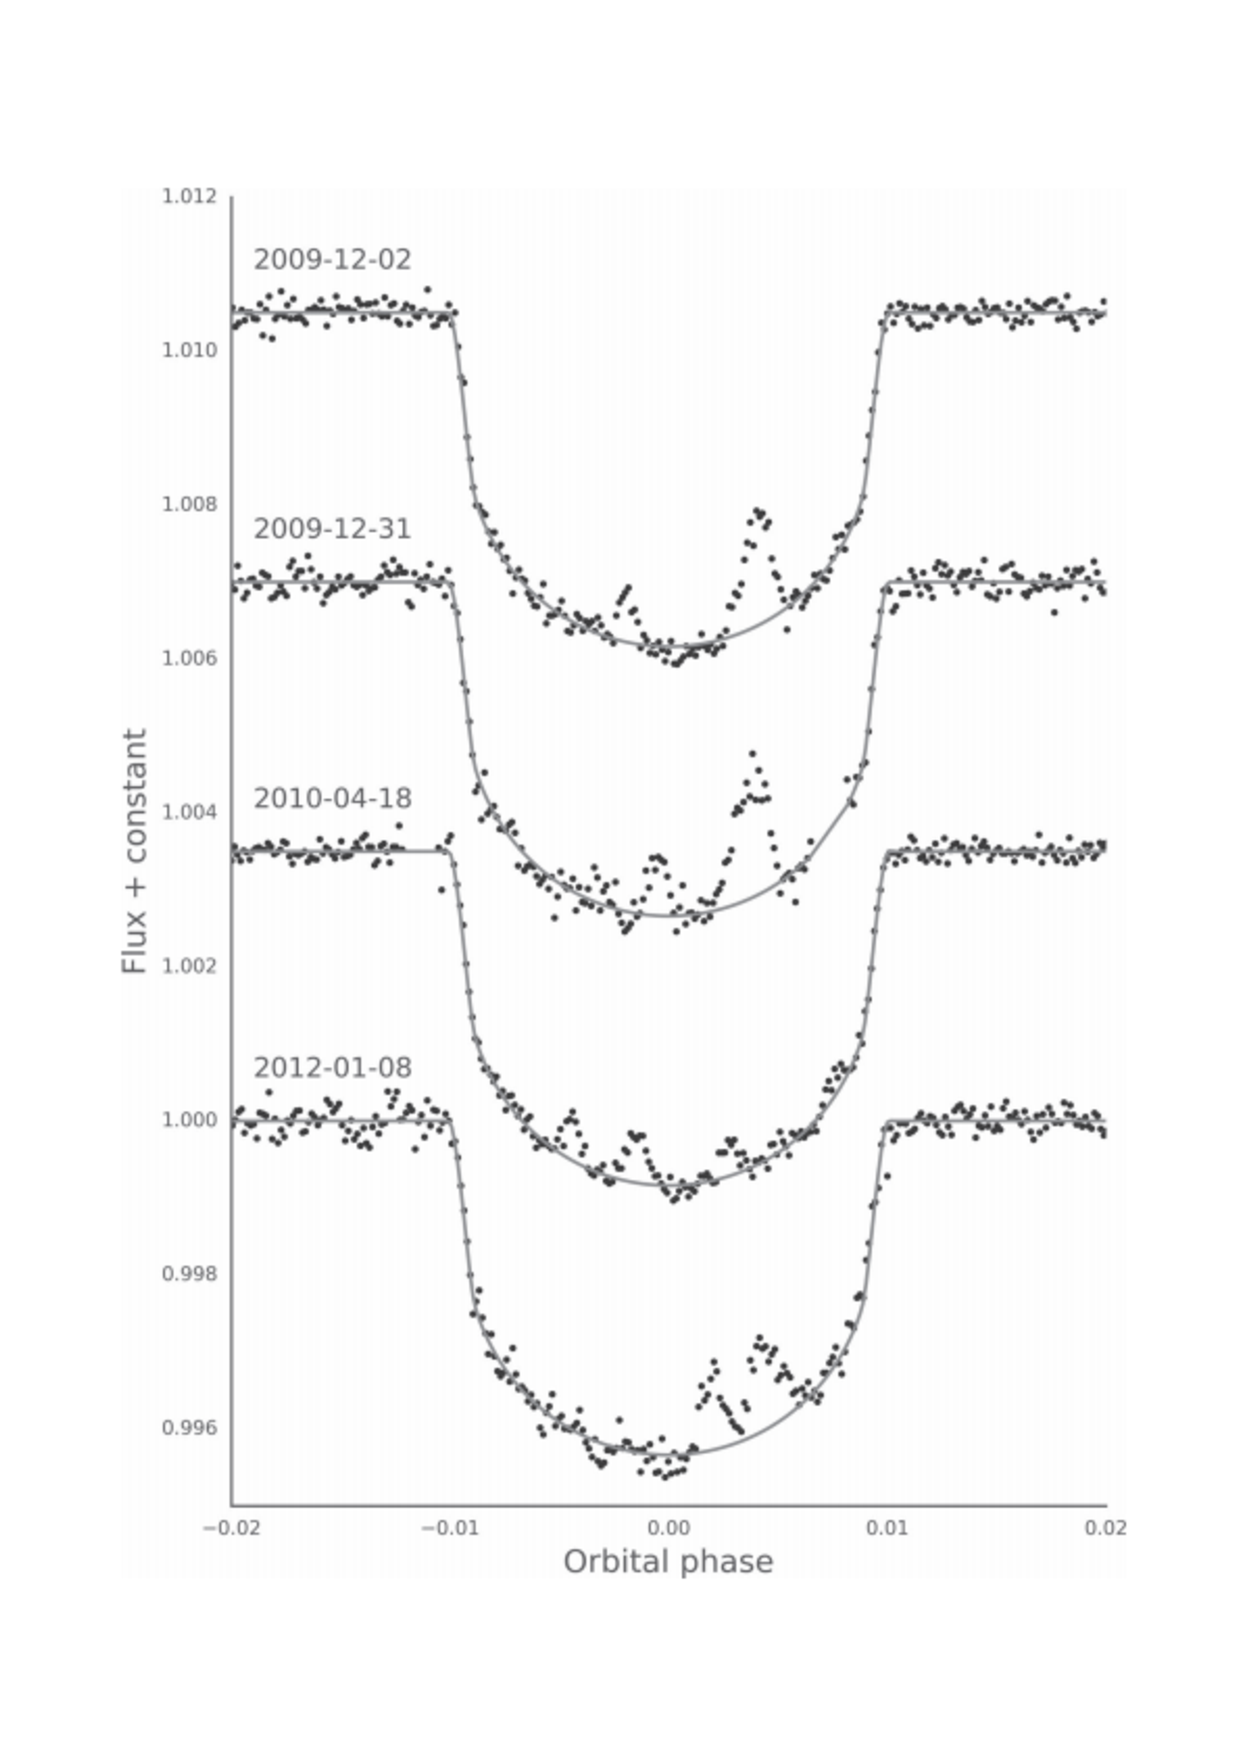
\includegraphics[scale=0.3]{Figures/1-Introduction/hatp_11_spots.pdf}
    \caption[Light curves with examples of starspot "bumps" in exoplanet transits]{Examples of Kepler transit light curves for HAT-11-11 b. Data points are Kepler fluxes and the curves indicate the best fir transit model. Positive "bumps" in the light curve is due to the exoplanet passing in front of a starspot. Image credit: \citet{Morris_etal_2017}}
    \label{fig:spot_occultation_example}
\end{figure}

There are other techniques that can be used to observe starspots such as Doppler imaging, however this technique is limited to fast rotators. A much more common way of observing starspots on slower rotators is through spot occultations by transiting exoplanets. Exoplanets are simply planets that orbit another star; transiting exoplanets pass in front of their host star and cause a small dip in the light curve of their host star. The transiting method has been the most successful way of discovering exoplanets since the launch of space telescopes such as Kepler which also provide a long baseline for observations. During the transit of any object, the flux lost is proportional to the intensity of the area occulted. When an exoplanet transits a starspot, a cooler region of the stellar surface is occulted and causes a positive flux anomaly in the transit light curve as shown in Figure \ref{fig:spot_occultation_example}.

\subsubsection{Chromospheric emission}
\label{chromospheric_emission_subsub}
As discussed previously we know that non-thermal heating caused by the magnetic field causes a temperature rise in the chromosphere. This results in emission reversals in certain spectral lines such as \caII (located at 3968.47 \AA \space and 3933.66 \AA \space respectively) which vary linearly with the magnetic field strength \citep{Frazier_1970}. This is a very useful tool to study the magnetic activity on other stars as these can be seen in a spectrum. The \caII lines have been studied for decades on other stars, starting with the Mount Wilson Observatory (MWO) project founded by O. Wilson to try and find analogous stellar cycles as the Sun through the monitoring of the \caII lines \citep{Wilson_1968}.

This project went on to build a new more efficient instrument known as the HK Photometer 2 \citep{Vaughan_etal_1978} which led to the introduction of the now standard S index for measurement of calcium emission. The S index takes a measurement of the flux within the \caII lines and normalises it by the flux in two continuum reference channels as shown in Equation \ref{Eq:s_index} where $N_{x}$ is the total counts in the relevant channel. Two 1.09 \AA \space wide triangular channels are centred on the \caII lines while the R and V channels are 20 \AA \space wide centred on 40001.07 and 3901.07 \AA respectively. Generally, S indexes from other spectrographs are calibrated to the Mount Wilson S index (hereafter, \Smw) as the value of the S index is dependent on the throughput of the spectrograph.

\begin{equation}
    S = \frac{N_{H} + N_{K}}{N_{R} + N_{V}}
    \label{Eq:s_index}
\end{equation}

There are some issues with using the S index to compare the calcium emission from stars with differing spectral types. For stars at an equal distance, the values of $N_{R}$ and $N_{V}$ will be larger for more massive stars and smaller for less massive stars. In addition to this, the 1.09 \AA \space channel for the \caII lines is wide enough to admit light that comes from the photosphere as well as the chromospheric component. This introduces a colour or mass dependency into the S index and therefore cannot be used to compare emission of stars with varying spectral types.

This colour/mass dependency was resolved by \citet{Noyes_etal_1984} who developed the chromospheric ratio \Rprime which is defined by Equation \ref{Eq:Rprime}; $\mathcal{F}$ represents the absolute flux in the H and K channels from chromospheric emission and $\sigma T_{eff}^{4}$ is the bolometric flux. Since the absolute fluxes are more difficult to calculate, \citet{Middelkoop_1982} determined an empirical relationship between the S index and the absolute fluxes known as $R_{HK}$. \citet{Noyes_etal_1984} improved upon this relation by determining the photospheric contribution ($R_{phot}$) as a function of $B-V$ colour and subtracting this from $R_{HK}$ to obtain $R^{'}_{HK}$ which is purely the chromospheric contribution.

\begin{equation}
    R^{'}_{HK} \equiv \frac{(\mathcal{F}_{H} + \mathcal{F}_{K})_{Chromo}}{\sigma T_{eff}^{4}} = R_{HK} - R_{phot}
    \label{Eq:Rprime}
\end{equation}

In order to calculate the \Rprime indicator from the \Smw, firstly Equation \ref{Eq:rhk} is used to convert the \Smw value into $R_{HK}$ value where $C_{cf}$ is the correction factor and is a function of the $(B-V)$ colour of the star as shown in Equation \ref{Eq:c_cf}. The photospheric contribution to the \caII spectral lines ($R_{phot}$) has also been calibrated as a function of $(B-V)$ colour of the star and is calculated by Equation \ref{Eq:rphot}.

\begin{equation}
    R_{HK} = 1.34{\times}10^{4}C_{cf}S_{MW}
    \label{Eq:rhk}
\end{equation}

\begin{equation}
    \log C_{cf} = 1.13(B - V)^{3} - 3.91(B-V)^{2} + 2.84(B-V) - 0.47
    \label{Eq:c_cf}
\end{equation}

\begin{equation}
    \log R_{phot} = -4.898 + 1.918(B-V)^{2} - 2.893(B-V)^{3}
    \label{Eq:rphot}
\end{equation}

One parameter that is not considered in the \Rprime indicator is metallicity, this will affect the depth of the convection zone within the star. The metallicity will change the interior opacity of the star, this then changes the point at which the convection zone starts. Metal-rich stars will have a deeper convection zone and thus have a longer convective turnover time ($\tau_{C}$). This also affects the shape of the \caII line profiles, metal-poor stars have shallower line profiles which mimics high levels of chromospheric fill-in making the star appear more active and younger than metal-rich stars \citep{Rocha-Pinto_Maciel_1998}.

Other spectral lines also include a chromospheric component including the $H-\alpha$ line (located at 6562.81 \AA), this is commonly used in studies of low-mass stars such as M dwarfs (e.g. \citealt{Newton_etal_2017}). This is due to the low level of continuum in the \caII region which makes calculation of the \Rprime indicator more difficult. Extensive research has been undertaken to investigate the correlation between \caII and $H-\alpha$ emission. A single one to one relationship does not exist between the two activity indicators and a wide variety of correlations have been found in other stars as seen in \citet{Cincunegui_etal_2007}. The large variation in correlation can be explained by how plage and filaments contribute to the \caII and $H-\alpha$ lines as suggested by \citet{Meunier_Delfosse_2009}.

\subsubsection{Coronal emission}
The age of stellar X-ray astronomy began in the 1970's with the detection of Capella (a G-type giant star) as the first stellar coronal X-ray source \citep{Catura_etal_1975}. The first main sequence star to be detected in X-rays was Alpha Centauri \citep{Nugent_Garmire_1978} and was identified as an inactive coronal source similar to our own Sun. The field was revolutionised when the Einstein telescope was launched in 1978 and made several key insights in stellar X-ray astronomy. Firstly, stars became one of the most prominent classes of cosmic X-ray sources as seen in \citet{Vaiana_etal_1981}; stars from the pre-main sequence, along the entire main sequence and even giant stars were detected in the X-ray regime. The X-ray luminosity and distribution along the main sequence could not be in agreement with the long favoured model for coronal heating - acoustic wave heating. Coronal X-ray emission was now interpreted as an effect of magnetic coronal heating. Lastly, stars that are otherwise similar showed large difference in X-ray luminosity if their rotation periods were different \citep{Pallavicini_etal_1981}. Since then many surveys of stellar coronae have been undertaken using X-ray telescopes (e.g. \citealt{Fleming_etal_1995,Schmitt_1997,Nebot_etal_2013,Wood_etal_2018}). Even in the early surveys, the sensitivity was sufficient enough to suggest a lower limit to the main sequence X-ray luminosity of a few times $10^{25}$ ergs $s^{-1}$ similar to that of solar coronal holes.

The first X-ray spectrum of a stellar corona was obtain of Capella by \citet{Cash_etal_1978} and correctly interpreted that the excess emission between 0.65 and 1 keV was due to an iron complex. Another element of modern coronal X-ray astronomy was introduced by \citet{Walter_etal_1978} when they realised that sub-solar abundances were needed to fit the coronal X-ray spectrum. Now with the introduction of Chandra and XMM-Newton telescopes, a new era in X-ray astronomy has begun with the technology needed to perform high-resolution spectral studies.

It is worth noting that while X-ray observations are more resource intensive (typically taken on the timescale of ks), they provide a direct link to the magnetic heating that causes the emission. X-ray luminosity does not have any strong dependencies on other parameters such as metallicity, thus making it a much more direct measure of magnetic activity. However, it is worth noting that during the solar cycle, the Sun's X-ray luminosity can be an order of magnitude higher or lower than the mean value.

\section{Ages of stars}
\label{Section:intro_ages}
Knowledge of stellar ages are useful in many different areas of astrophysics; for very young stars (i.e. $<$ 100 Myr), if we want to understand the timescale of planet formation then we must observe such systems and know the stellar age. If we observe enough systems with various stages of planet formation then this information can be fed back into theoretical models. In terms of galactic history, it is paramount that we can assign stellar ages for individual stars to understand the formation of the galaxy. This is particularly true when considering low mass stars that are able to live long enough to be present for all epochs of star formation. Another example of how stellar age is an important parameter to obtain is to consider the evolution of the Sun (both in the past and future); to fully understand the Sun we must look at other solar-like stars at different stages in their evolution. These type of studies will give us greater insight into what conditions were like when life was forming on Earth and how the Sun will evolve in the future. When considering exoplanet systems, in order to deepen our knowledge of the dynamics of such systems or the potential migration that has taken place (in the case of Hot Jupiters) we need to know the age of the star. Stellar ages are particularly important when it comes to the search for life outside of our own solar system as they will help us understand the timescale needed for such biological evolution. These are just a few of the many reasons why stellar ages are important in astrophysics, yet how do we calculate these ages? This is the question I will address in this section by outlining various methods of determining stellar ages and discussing the advantages and disadvantages of each one.

The Vogt-Russel theorem states that the structure of the star can be uniquely determined by its mass and chemical composition; other factors may play a role (such as rotation, magnetic field or companions) but mass and composition dominate. The age of a star can influence the state of the star as over time the chemical composition of the star will change, however, this is due to nuclear fusion taking place in the star and the stellar age is not the direct agent of this change. Consequently, we cannot directly measure a star's age but rather it must be estimated or inferred. The only accurate and precise stellar age known is for our own Sun, but this value is not calculated from observing the Sun but rather through the study of meteorites. Meteorites contain long-lived radioactive isotopes of elements that can be used to age the material, since meteorites are the left over debris from the planet formation process it follows that it should have the same age as the solar system and the Sun. The age of the Sun is found to be $4.57 \pm 0.02$ Gyr  where 1 Gyr is equivalent to a billion years \citep{Bahcall_etal_1995}. This is known as a fundamental age as the physical process behind the method is fully understood. In this section I will describe some common methods used to determine the ages of stars and in particular the ages of single stars that are on the main sequence as these stars are the focus in this thesis. For a more thorough review of different methods to determine ages of stars see \citet{Soderblom_2010}.

\subsection{Semi-fundamental ages}
While the only fundamental age known is for our own Sun, there are some methods that produce semi-fundamental ages i.e. methods where the physical process is understood but must invoke a few (well-founded) assumptions. One of these is known as nucleocosmochronometry and uses the presence of long-lived isotopes in stellar spectra to date the stars. Typically the isotopes used are $^{238}$U and $^{232}$Th which have half-lives of 4.47 and 14.05 Gyr respectively. However, these spectral lines can only be measured in metal-poor stars where the weak isotope lines can be measured within the presence of other line blends. Therefore the method is used to date the oldest stars that formed at the earliest epoch in the galaxy. While the physical process that underlies this method (i.e. nuclear decay) is known, the initial abundance of the isotope within the star is an unknown quantity thus making the age a semi-fundamental value. The initial abundance of the isotope is scaled from other r-process elements assuming production rates from these other elements being measured. These r-process elements are all heavier than Iron and are created in the aftermath of core-collapse supernovae or binary neutron star mergers. \citet{Ludwig_etal_2010} quantified the uncertainties associated with this age-dating method and found that the accuracy is poor when considering a single star; uncertainties of $\approx$ 2 Gyr are common when considering observation uncertainties only. Improved results should come from larger samples of stars (e.g. globular clusters or dwarf galaxies) where a larger sample of old, metal poor stars are found (see e.g.\citealt{Hansen_etal_2018}). 

Another semi-fundamental age dating method uses kinematics; in this method the motion of a group of stars is traced into the past and determines when they were in closest proximity to each other which is then assumed to be the time of formation. While this method is independent of any stellar physics as it relies mainly on astrometry, it requires high-quality kinematics data in all three dimensions including parallax and radial velocities. In addition to the full 3-D kinematic data, good accuracy is needed therefore this method is predominately used for nearby groups (e.g. see \citealt{Makarov_2007}). Typically, using kinematic data, we cannot go back further than 20 - 30 Myr due to the uncertainties in the input parameters. Also, some young groups appear to have very little net expansion \citep{Mamajek_2005} therefore determining the time at which the group of stars was closest together is ill-defined. However, the fundamental limitation on this method is the evolution of galactic orbits over time; as stars and clusters orbit about the galaxy they encounter massive objects that can disrupt their orbits and create field stars, for example. The timescale for such interactions with these objects is $\approx$ 200 Myr \citep{Janes_Phelps_1994} which is similar to the galactic rotation period. Therefore, only young stars can dated using this method as it can be assumed that their galactic orbits are undisturbed.

\subsection{Model dependent ages}
As discussed in the previous section, there are some methods that can determine semi-fundamental ages but can only be applied to a limited number of stars. Consequently, in order to determine ages for other stars, methods must be used that are based on stellar models.

\subsubsection{Isochrones}
One such model dependent method is the use of isochrones on a Hertzsprung-Russel Diagram (HRD). An isochrone is defined as a line on a diagram connecting points to the same time; in the stellar case this represents a population of stars (of different masses) with the same age. A HRD plots the absolute magnitude as a function of stellar temperature and shows the various stages of a stars evolution depending on the position within the diagram. The main sequence on the HRD goes from the top left to the bottom right of the diagram and shows the stars while they are in their hydrogen burning phase (i.e. nuclear fusion of hydrogen into helium is occurring within the core). As the star evolves and uses up the hydrogen supply within the core, they move to the right on the HRD becoming subgiants and eventually giants. However, the age at which stars evolve off the main sequence is dependent on the mass of the star - more massive stars use up their hydrogen supply quicker than low mass stars. This technique has been successfully used to date open clusters, as we can observe the full population of stars and determine the main sequence turn off. If the masses of the stars that have evolved off the main sequence are known then stellar models can be used to determine the age of the cluster. An example of a HRD diagram with several isochrones (of varying ages) is shown in Figure \ref{fig:OC_isochrone_example}.

\begin{figure}
    \centering
    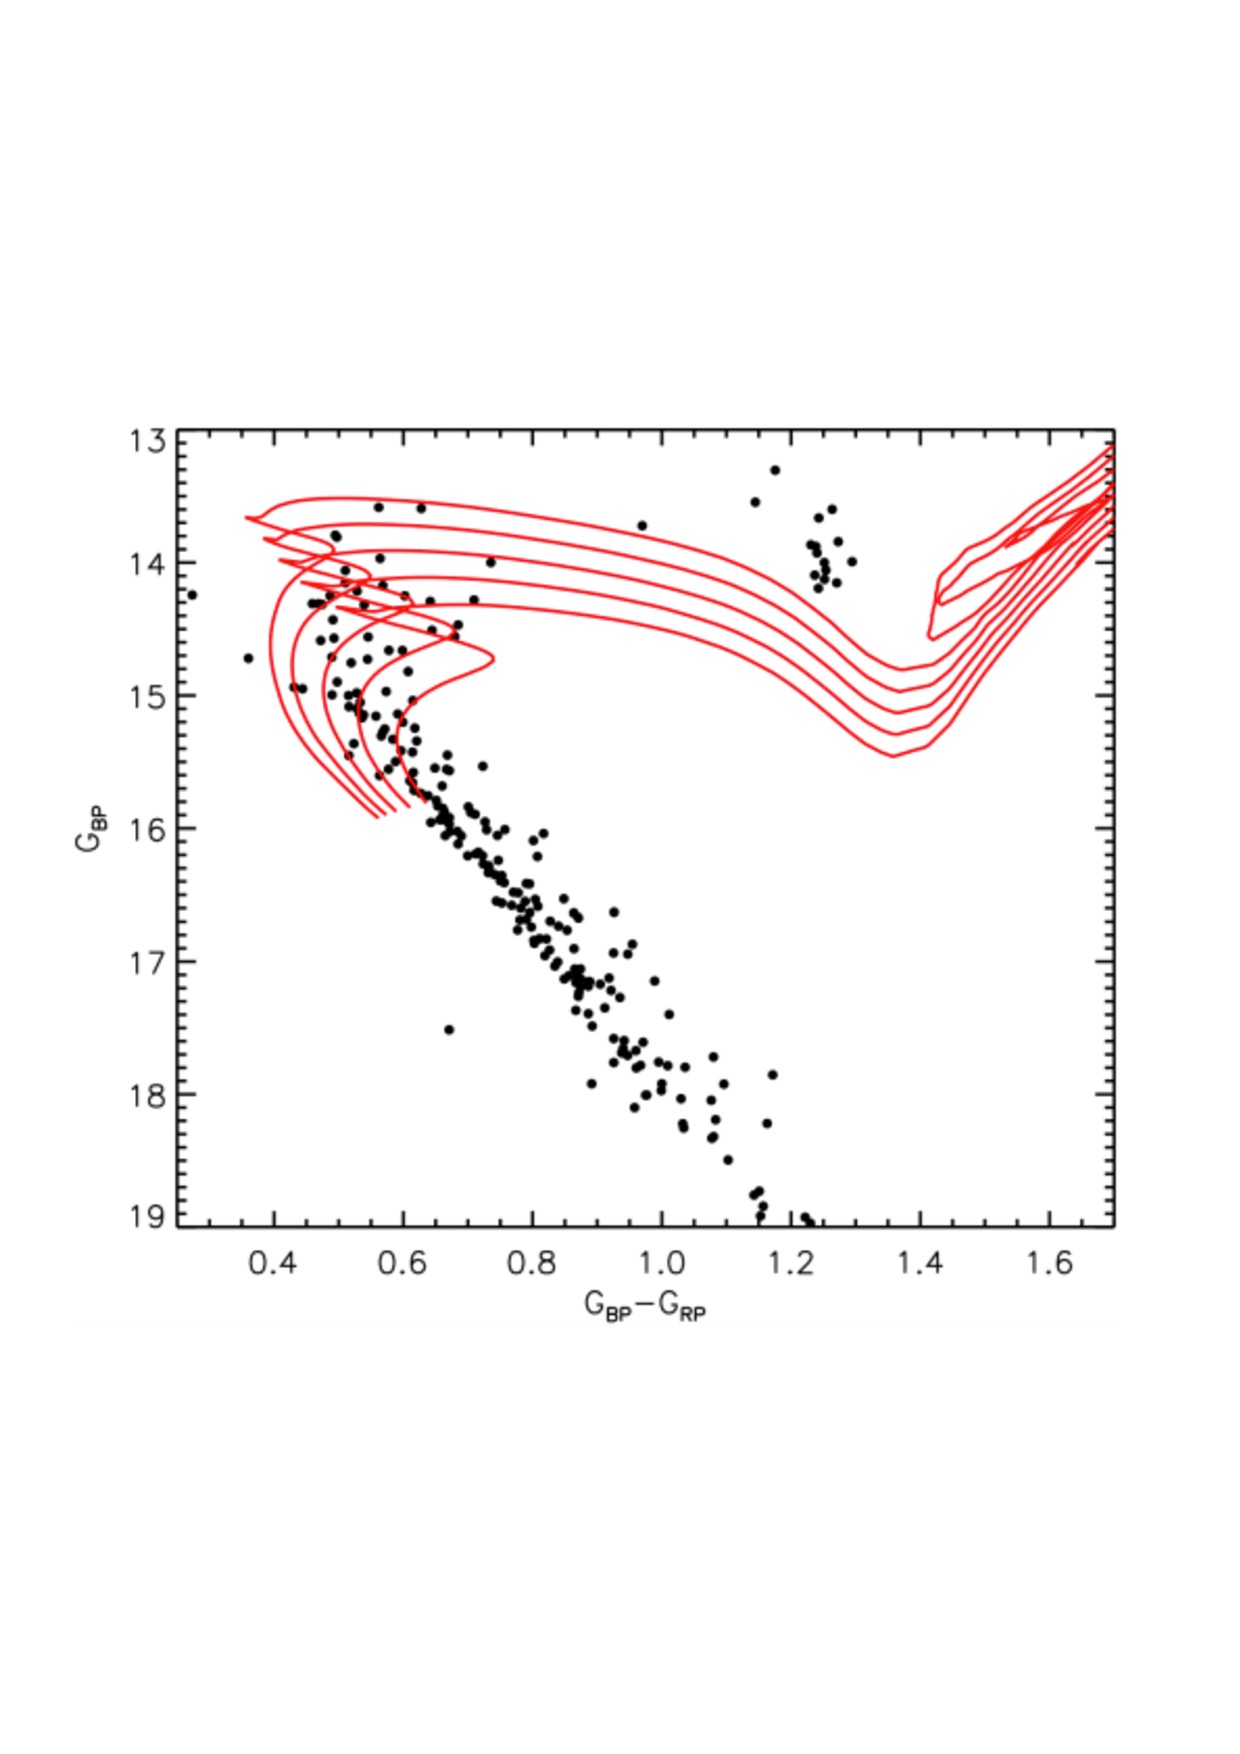
\includegraphics[scale=0.45]{Figures/1-Introduction/gaia_OC_example.pdf}
    \caption[Example of colour-magnitude diagram for a cluster used to fit isochrones]{Example of a colour-magnitude diagram (observational equivalent of HRD) for NGC 2818 as seen in \textit{GAIA} filters. Red lines indicate isochrones with ages between $log$ t = 8.85...9.05 (in steps of 0.05). Image credit: \citet{Bastian_etal_2018}}
    \label{fig:OC_isochrone_example}
\end{figure}

Isochrones have also been used to determine ages of single field stars, however since a distributed fit is not possible like in the cluster data, a different method is used to analyse the data. Isochrones have complex shapes, particularly near the main sequence turn off, and multiple isochrones may pass through the same point on the HRD. This creates a degeneracy when trying to determine the ages of field stars since only one data point exists. Some of this degeneracy can be removed when either the abundances are known or if the star is in a binary system.

In order to calculate an age for a field star using the isochrone method, the best estimate of the temperature, metallicity and luminosity (along with uncertainties) must be known in order to minimise the degeneracy. One method is to interpolate among model isochrones to the location of the star in the HRD. Yet this method introduces bias because of the complex shapes of the isochrone and the non-uniform spacing between the isochrones. The majority of stars should fall near the zero-age main sequence (this is the location in the HRD that stars begin on the main sequence) but uneven spacing in isochrones results in biases towards older ages. This bias is clearly seen in one of the earliest attempts using this method \citep{Perrin_etal_1977} as most of the ages were found to be greater than 10 Gyr. In recent years, more sophisticated methods have been applied such as Bayesian methods to reduce the effect of these biases (e.g. \citealt{Takeda_etal_2007}). However, errors typically have values between 20\% - 50\% before taking into account any systematics.

\subsubsection{White dwarf cooling}
An alternative method uses the presence of white dwarfs to age stars in a cluster and/or a binary system. White dwarfs are the final remnant cores of low and intermediate stars after they have used up their hydrogen supply within the core and completed their evolution as giant stars. White dwarfs are highly dense objects typically with masses of 0.6 M$_{\odot}$ with radii comparable to the earth ($\approx$ 7000 km) \citep{Madej_etal_2004} and made up predominantly of product elements from Helium fusion - carbon and nitrogen. They are particularly important astronomical objects to study as they are representative of the stellar population as a whole since the majority of stars will become white dwarfs.

Since white dwarfs are the remnant cores of stars they no longer undergo nuclear fusion. Instead, they are powered by the internal energy stored in the thermal motions of the ions and gradually cool over time \citep{Mestel_1952} resulting in observable changes in luminosity and temperature. This results in the ability to have a white dwarf isochrone, but to determine the ages of these white dwarfs more knowledge is needed in comparison with the usual isochrone discussed previously. The white dwarf cooling models are relatively well understood and can inform us of the time that it has taken for the white dwarf to cool to a particular temperature, but this only pertains to the white dwarf portion of the stellar life. In order to obtain the age of the white dwarf, information is needed about the progenitor star and this is usually obtained through an initial-final mass relationship (IFMR). This relationship links the mass of the white dwarf to the initial mass of the star prior to mass loss on the asymptotic giant branch and relies on stellar models. The relationship is still an active topic of research as the latest stages in a star's life are extremely sensitive to many parameters and white dwarfs are even used to constrain the models behind the IFMR \citep{Cummings_etal_2018}. In order to calculate the mass of a white dwarf, spectroscopic observations are needed to calculate the effective temperature and surface gravity (log(g)). Once the mass of the white dwarf is known then one can use the IFMR to infer the mass of progenitor star. Lastly, stellar evolution codes can provide the main sequence lifetime of the progenitor star that can be added to the white dwarf cooling time to obtain the age of the white dwarf.

This technique has been used to determine ages for clusters, particularly globular clusters in recent years (e.g. \citealt{Torres_etal_2015}) giving us insight into the true ages of the oldest stars in our galaxy. It is particularly useful to compare the ages determined from white dwarfs to those from main sequence turn off ages in clusters as seen in \citet{Garcia-Berro_etal_2010}. This study's motivation was to try and explain the discrepancy between the ages from the two methods by adding a predicted theoretical mechanism (crystallisation of a product of helium burning) which would delay the cooling phase of a white dwarf. As predicted, by adding in this mechanism the age discrepancy was resolved. Even clusters that have generally accepted ages like the Hyades are being studied using white dwarfs \citep{Salaris_Bedin_2018}. However, this technique has also been used to age stars in binary systems with a white dwarf companion (e.g. \citealt{Liebert_etal_2013}) and even the galactic halo \citep{Kilic_etal_2019}. It is the use of the method in these environments outside of clusters where no other age dating method could be invoked that makes this such a useful tool if a white dwarf is present.

\subsubsection{Asteroseismology}
Asteroseismology is the study of stellar oscillations in order to gain insight into the interior layers of a star and it is particularly useful for determining fundamental parameters of a star such as mass, effective temperature, log(g) and even age. In the context of stellar ages, it has been revolutionary for determining ages of isolated, old main sequence field stars. The stellar oscillations are caused by waves within the interior of the star interfering with one another to generate standing waves. There are two types of oscillations and they are defined by the restoring force that acts upon them; gravity (g) modes where buoyancy is the restoring force and pressure (p) modes where gradients of pressure act as the restoring force. The main advantage of studying asteroseismology is that since the oscillations originate from within the interior of the star then it allows information about this area to be obtained.

In the early 1960's, the discovery and interpretation of solar oscillations led to the development of the helioseismology field (for a review see \citealt{Christensen-Dalsgaard_2002}). In the Sun, we see p modes that are  driven stochastically, intrinsically stable and created by turbulent motions in the sub-surface convection zone \citep{Samadi_Goupil_2001}. These oscillations are relatively high frequency - in the range of 1000 - 5000 $\mu$Hz which corresponds to 17 - 3 minute periods. These types of oscillations are generally referred to as solar-like oscillations, however they can occur in non-solar-like stars (such as giant stars), the stars simply need to be cool enough to have an outer convection zone. Gravity or g modes are generally found in other stars such white dwarfs and stars that pulsate such as some B stars. Since these modes are generated deep within the core, they are strongly dampened by convective motion and are typically not seen in solar-like stars thus the rest of this section will concentrate on p mode oscillations.

The geometrical structure of oscillation modes are described as a spherical harmonic which assumes spherical symmetry in stars. There are three important integers to consider; firstly $n$ which is the radial order and specifies the number of nodal shells in the standing wave. Secondly, $l$ which measures the total number of nodal lines on the surface. Modes with a value of $l=0$ are known as radial modes and $l$ values greater than this are known as non-radial modes. Since the surfaces of stars are not resolved, typically only modes with values of $l$ less than four are observable. The third integer is $m$, the azimuthal order and has values from $+l$ to $-l$. The oscillation frequency does not depend on $m$ unless spherical symmetry is broken, for example in the presence of a magnetic field or the star is rotating. Therefore, for a rotating star with a mode with given $n$ and $l$ values, there will be a split in the frequency of the mode into a multiplet with $2l + 1$ component (one for each value of $m$). It is possible to determine the rotational frequency of a star as it is proportional to the frequency separation between these components.

Space missions such as CoRoT and Kepler have revolutionised the asteroseismology field with exquisite precision light curves and long timescales. For example, one of the early surveys for asteroseismology with Kepler by \citet{Chaplin_etal_2011} looked at over 2,000 main sequence and giant stars in short cadence mode and detected solar-like oscillations for approximately 500 stars. Fourier analysis is performed on the Kepler light curves to obtain a power spectrum that contains information on the frequencies of any oscillations present. Figure \ref{fig:power_spectrum_example_sun} shows an example for the Sun, panel (a) shows the full power spectrum and panel (b) shows an zoomed in portion with labelled modes and frequency separations. From the power spectrum we can define some variables that are key in asteroseismology studies; in panel (a) we see that the peak heights create an envelope which can be used to define $\nu_{max}$ - the frequency of maximum power and has a value of 3,100 $\mu$Hz for the Sun. The next parameter that can be defined is $\Delta \nu$, the large frequency separation and is define as the spacing between consecutive radial overtones (i.e. modes with a given $l$ whose $n$ values differ by one). The large frequency separation has a value of 135 $\mu$Hz in the Sun. The last parameter that can be calculated is the small frequency separations (e.g. $\delta \nu_{0,2}$); these are frequency separations between close pairs with a difference of two in $l$ value and difference of one in $n$ values as shown in panel (b) of Figure \ref{fig:power_spectrum_example_sun}. An additional small frequency separation can be defined ($\delta \nu_{0,1}$) as the $l=1$ modes do not fall exactly half way between the $l=0$ modes. Therefore, $\delta \nu_{0,1}$ is the amount by which the $l=1$ mode are off set from the midpoint of the $l=0$ modes.

\begin{figure}
    \centering
    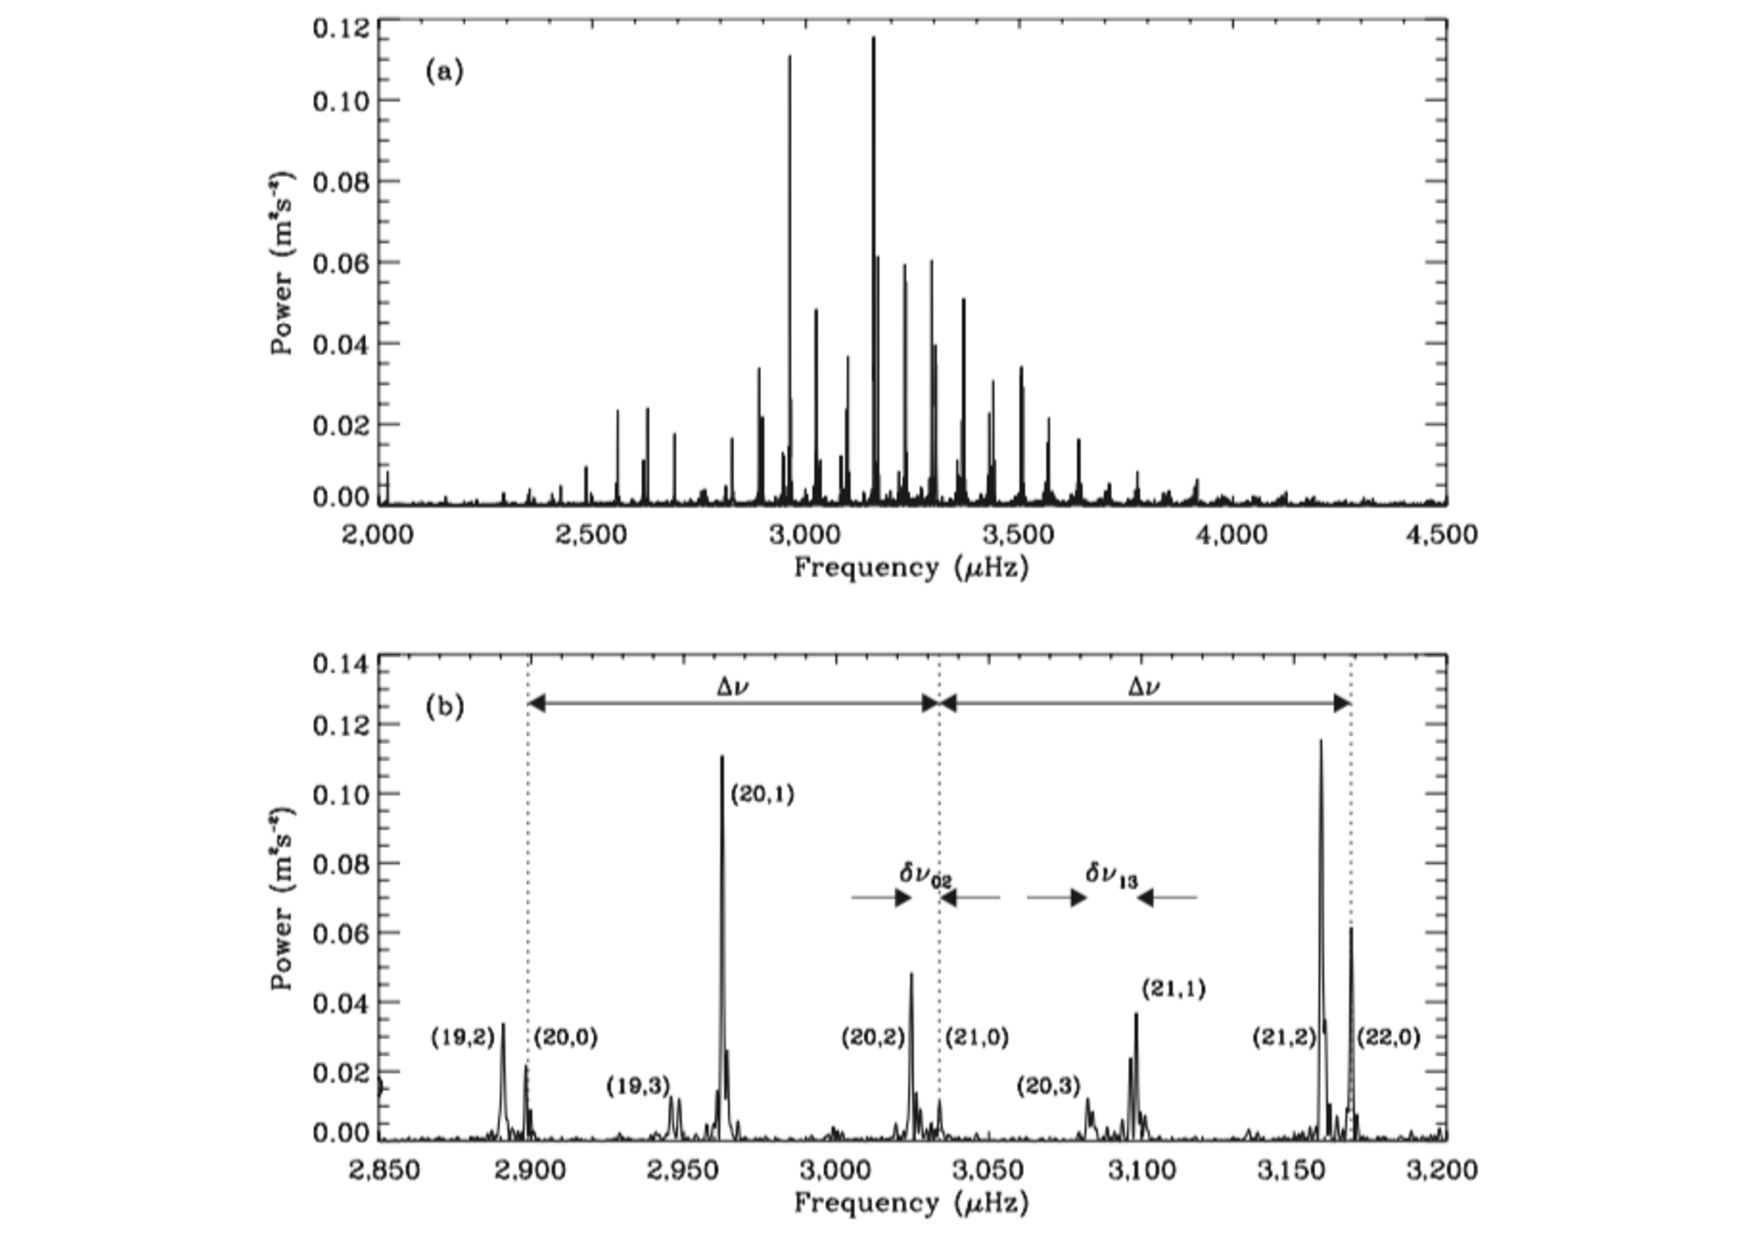
\includegraphics[scale=0.5]{Figures/1-Introduction/power_spectrum_sun.pdf}
    \caption[Example of solar power spectrum from which asteroseismic analysis can be conducted]{Panel (a) shows the solar power spectrum from ten days of disk-integrated velocity measurements with the BiSON instrument. Panel (b) shows a close-up labelled with (n,l) values for each mode. Dotted lines show the radial modes, and the large and small separations are indicated. Image credit: figure 3.1 from \citet{Palle_Esteban_2014}}
    \label{fig:power_spectrum_example_sun}
\end{figure}

While the parameters defined above come from observations, theoretical studies give physical meaning to these parameters. \citet{Brown_etal_1991} suggested that $\nu_{max}$ might be a a fixed fraction of the acoustic cut-off frequency. The cut-off frequency is defined as a boundary where energy flowing in the system becomes reduced. The acoustic cut-off frequency can be defined by Equation \ref{Eq:acoustic_cut_off_eq} where $c_{s}$ is the speed of sound and $H$ is the density scale height. An isothermal approximation of Equation \ref{Eq:acoustic_cut_off_eq} is taken to be $\nu_{ac} \propto \frac{c_{s}}{H}$ which is also proportional to the frequency of maximum power, $\nu_{max}$.

\begin{equation}
    \nu_{ac} = \left(\frac{c_{s}}{4\pi H}\right)^{2}\left(1 - 2\frac{dH}{dr}\right)
    \label{Eq:acoustic_cut_off_eq}
\end{equation}

Assuming the system is adiabatic and that the ideal gas law applies then the speed of sound squared will be proportional to the temperature. By substituting this and $H \propto \frac{T}{g}$ (which comes from the definition of the scale height), Equation \ref{Eq:v_max_eq} is obtained \citep{Kjeldsen_Bedding_1995}. Note that since oscillations are observed in the photosphere, it is reasonable to assume that the temperature is close to the effective temperature of the star. This equation shows that with a prior on the effective temperature of the star, the surface gravity of a star can be obtained from the measurement of $\nu_{max}$.

\begin{equation}
    \nu_{max} \propto g(T_{eff})^{-\frac{1}{2}}
    \label{Eq:v_max_eq}
\end{equation}

Theoretical calculations using asymptotic theory (e.g. \citealt{Christensen_Dalsgaard_1988}) shows that the large frequency separation, $\Delta\nu$, can be defined as the inverse of the sound travel time thorugh the star as shown in Equation \ref{Eq:theoretical_large_freq_separation}.

\begin{equation}
    \Delta\nu \simeq \left(2 \int_{0}^{R} \frac{dr}{c_{s}} \right)
    \label{Eq:theoretical_large_freq_separation}
\end{equation}

If Equation \ref{Eq:theoretical_large_freq_separation} is integrated from the centre to the surface of the star and a substitution for the speed of sound is made (assuming adiabatic conditions) then Equation \ref{Eq:large_freq_step_one} is obtained. $\langle T \rangle$ is the average internal temperature.

\begin{equation}
    \Delta\nu \propto \frac{\sqrt{\langle T \rangle}}{R}
    \label{Eq:large_freq_step_one}
\end{equation}

Finally, a substitution can be made for the average internal temperature where $\langle T \rangle \propto \frac{M}{R}$ which is derived from the virial theorem. This leads to Equation \ref{Eq:large_freq_final_eq} where $\langle \rho \rangle$ is the mean stellar density. Thus the measurement of the large frequency separation leads to the calculation of the mean stellar density.

\begin{equation}
    \Delta\nu \propto \left(\frac{M}{R^{3}} \right)^{\frac{1}{2}} \equiv \sqrt{\langle \rho \rangle}
    \label{Eq:large_freq_final_eq}
\end{equation}

Lastly, the small frequency separation is related to the age of the star \citep{Ulrich_1986}. \citet{Christensen_Dalsgaard_1984} noted that some frequency differences were dependant on stellar age due to the conversion of hydrogen into helium and the attendant reduction in the speed of sound near the core. Another useful diagnostic tool in asteroseismology is the C-D diagram, first introduced by \citet{Christensen_Dalsgaard_1984}, which plots the small frequency separation as a function of the large frequency separation. One such example is shown in Figure \ref{fig:CD_diagram_example} from \citet{White_etal_2011}, which shows a sample of stars with model tracks for mass and age. In the top right of the plot (corresponding to the main sequence phase), these tracks are sufficiently spread out that a mass and age can be determined for these stars. However, as stars evolve off the main sequence the model tracks converge for the subgiant and red giant evolutionary phases. One disadvantage to this method is that the model tracks depend on the metallicity, thus to ensure the most accurate parameters the metallicity of the star must be known.

\begin{figure}
    \centering
    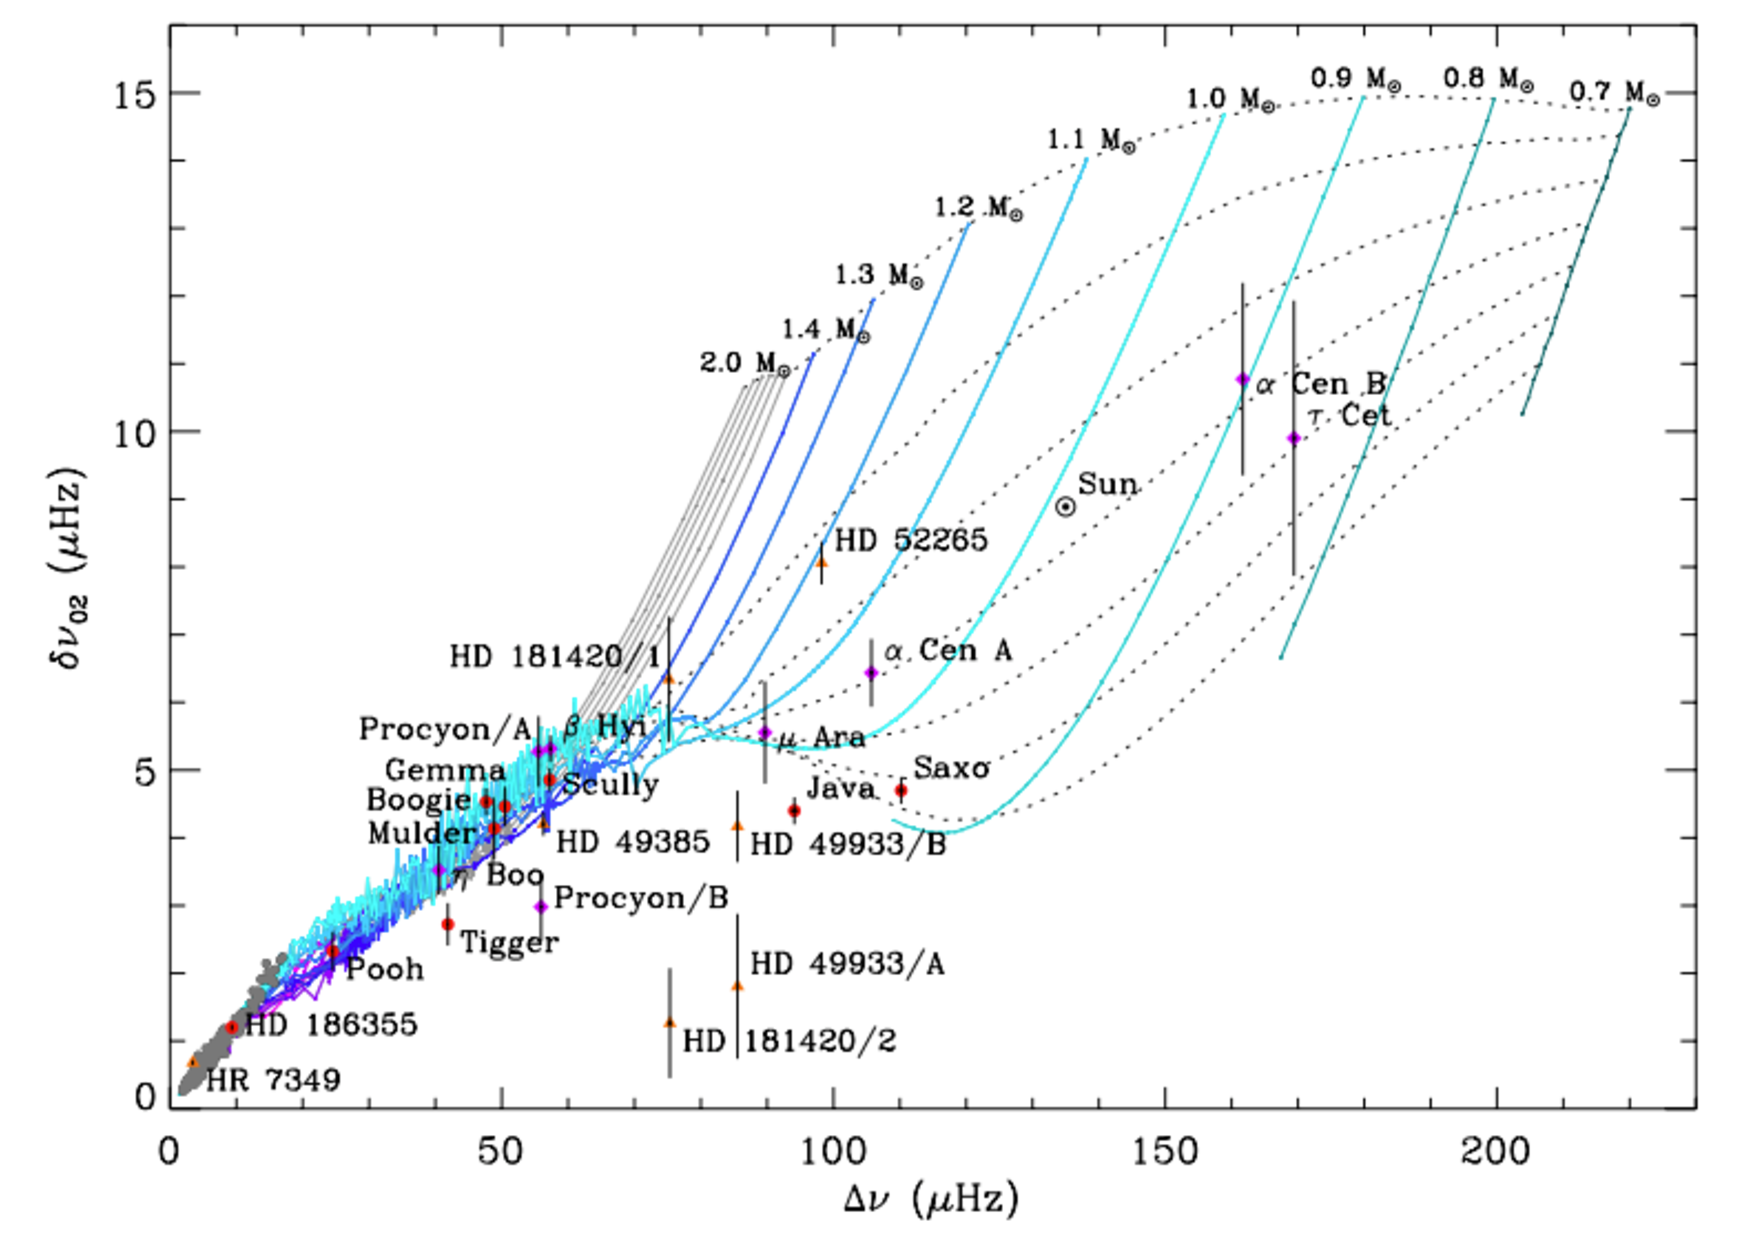
\includegraphics[scale=0.4]{Figures/1-Introduction/C-D_diagram.pdf}
    \caption[C-D diagram that can be used to age stars from asteroseismic parameters]{C-D diagram, with model tracks for near-solar metallicity (Z$_{0}$ = 0.017). Tracks increase in mass by 0.1 M$_{\odot}$ from 0.7 M$_{\odot}$ to 2.0 M$_{\odot}$ as labelled. Dashed black lines are isochrones, increasing by 2 Gyr from 0 Gyr (ZAMS) at the top to 12 Gyr at the bottom. Stars shown were observed using CoRot, Kepler or using ground telescopes. Image credit: \citet{White_etal_2011}}
    \label{fig:CD_diagram_example}
\end{figure}

As previously mentioned, asteroseismology has been revolutionised by space telescopes such as CoRoT and Kepler as they have greatly increased the number of stars with detected solar-like oscillations \citep{Chaplin_etal_2011}. Initially, the global asteroseismic parameters were used alongside complementary photometric and spectroscopic data to estimate stellar parameters \citep{Chaplin_etal_2014}. However, as the baseline for observations from Kepler increased and the signal to noise ratio become sufficient to study the individual frequencies, the precision of the stellar parameters also increased (e.g \citealt{Silva_Aguirre_etal_2015}). Figure \ref{fig:VSA_legacy_uncertainties} shows the distribution of uncertainties for the mean stellar density, radius, mass and age from a number of different pipelines for the Kepler LEGACY sample \citep{Lund_etal_2017}. This sample represents some of the highest signal to noise asteroseismic data that is currently available and we see that typical uncertainties in age are on the order of 10\%, which is a vast improvement on any other age dating method. With current and future space mission such as TESS \citep{Ricker_etal_2015} and PLATO \citep{Rauer_etal_2014}, both of which will further increase the number of stars with detected solar-like oscillations, the future looks bright for asteroseismology.

\begin{figure}
    \centering
    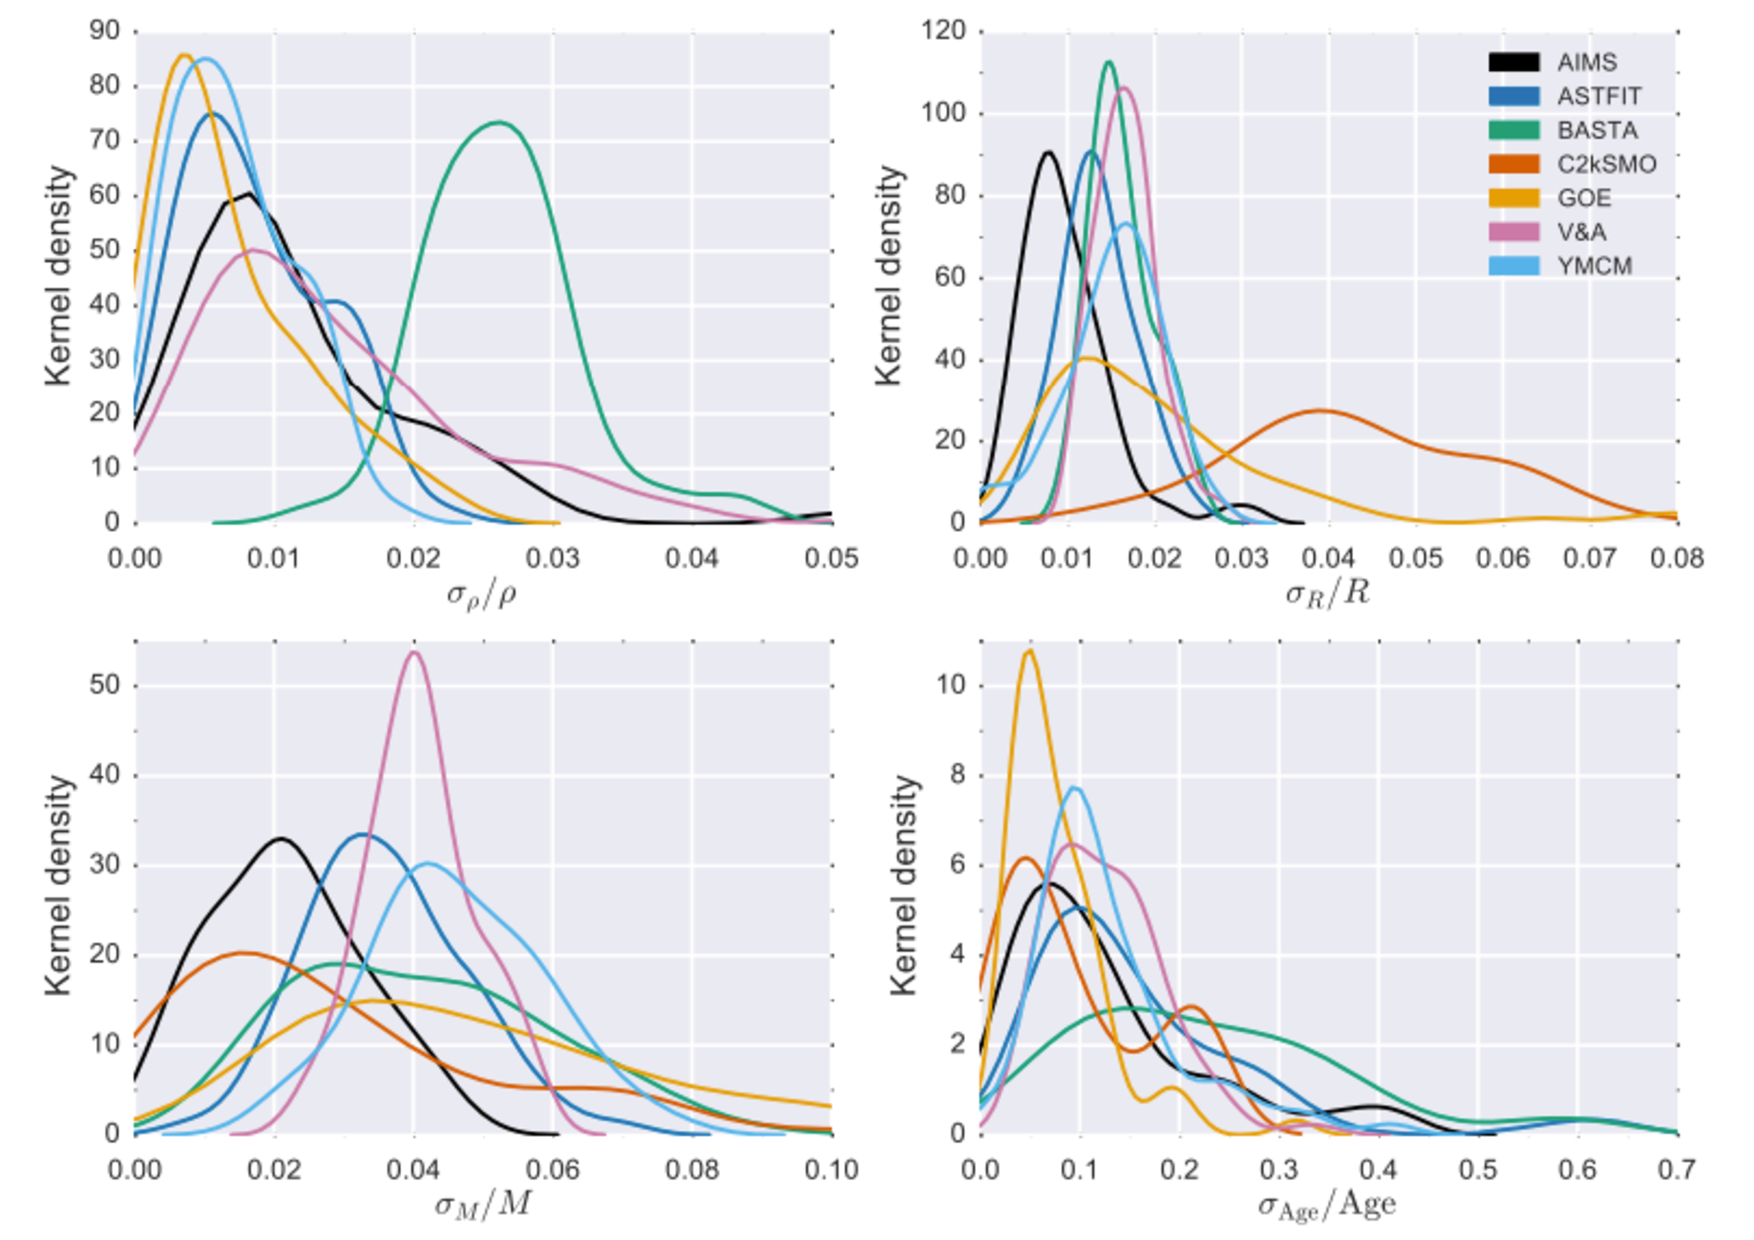
\includegraphics[scale=0.4]{Figures/1-Introduction/silva_aguirre_2017_legacy.pdf}
    \caption[Distributions of uncertainties in asteroseismically determined parameters]{Distributions of uncertainties of various stellar parameters for the whole Kepler LEGACY sample from a number of different pipelines. These stellar parameters are density, radius, mass and age. Image credit: \citet{Silva_Aguirre_etal_2017}}
    \label{fig:VSA_legacy_uncertainties}
\end{figure}

Yet like any other method, asteroseismology also has its disadvantages. For example, there is evidence that the magnetic activity of the star affects the detection of solar-like oscillations \citep{Chaplin_etal_2011_stellar_activity} suggesting that magnetic activity inhibits the amplitude of such oscillations. In addition to this, the intrinsic amplitude of the oscillations means that they are easier to detect in early-type and more evolved stars \citep{Houdek_etal_1999}. Therefore such asteroseismic samples may be biased to low activity and more evolved stars which must be taken into consideration. Also, in order to gain the highest signal to noise asteroseismic data (and therefore the most precise stellar parameters), observations must be taken over a long period of time. This will only be possible for a fraction of the stellar population, therefore how can we determine ages for stars that have not been studied using asteroseismology?

\subsection{Empirical age relations}
An alternative way of determining ages for stars is to use empirical age relationships. This method takes a stellar parameter and shows how it evolves in time therefore making it possible to infer an age for a star from a single parameter. In these relationships, a plausible physical mechanism works to cause the change in the stellar parameter over time but the exact physics underlying it are not fully understood. Furthermore, these relationships must first be calibrated by studying these stellar parameters for stars with known ages. Ages are typically calculated using one of the model-dependent methods described previously making these empirical relationships secondary to the model-dependent methods of determining ages. However, they can provide an estimate of the star's age where no other method can be used.

As discussed previously, in solar-like and low mass stars there exists a dynamo mechanism that links the rotation and magnetic field of the star. Through magnetic braking over the main sequence lifetime of a star, we expect the star to lose angular momentum which causes an increase in the observed rotation period of the star and consequently a decrease in the overall magnetic activity of the star. For this reason rotation and magnetic activity are commonly used in these relationships.

It is these empirical age relationships (particularly the age-activity relationship) that are the focus of the research presented in this thesis. While they may be a secondary method of determining ages in comparison to the model-dependent ages, they are important in the understanding of the physical processes that underpin them. From constraining the age-activity relationship, we gain new information in how the stellar wind and dynamo change over the main sequence lifetime of a star. In the next chapter, an overview of previous work concerning magnetic activity and rotation as function of age will be discussed.

\section{Structure of Thesis}
In this thesis I present a study of the magnetic activity of solar-like and low-mass stars as the evolve on the main sequence phase. This study includes an investigation into the relationship between X-ray luminosity and stellar age using asteroseismic ages and observations from X-ray telescopes. I also conduct an investigation in the evolution of chromospheric emission, primarily from the \caII spectral lines, again using asteroseismic ages. An additional investigation is conducted into how these activity indicators relate to the stellar rotation period. In this chapter I have given an overview of some of the key aspects needed in order to fully appreciate the underlying mechanisms at work in the age-activity-rotation relationship.

In Chapter 2 I will give an historical overview of the previous work that has been conducted concerning the age-activity-rotation relationship, the current limitations and regimes where the relationship is not fully understood. Chapter 3 is a study on the age-activity relationship using X-ray observations and asteroseismic ages for stars older than a gigayear. Chapter 4 details an investigation into the chromospheric emission as a function of age using optical spectra data and asteroseismic ages. Chapter 5 attempts to piece together the age-activity relationships determined in previous chapters with rotational data. Finally, in Chapter 6 I will give a summary of the main conclusions of my work and highlight the potential avenues that could be investigated with future work.
